\chapter{Aplicaciones de la derivada}

En el cap\'{\i}tulo anterior se interpret\'{o} el valor de la derivada de una
funci\'{o}n en un punto, como la pendiente de la recta tangente a la
gr\'{a}fica de la funci\'{o}n en dicho punto. No es extra\~{n}o entonces
acudir a la derivada para analizar la gr\'{a}fica de una funci\'{o}n en un
intervalo dado. En el presente cap\'{\i}tulo se usar\'{a} la derivada como
instrumento para dicho an\'{a}lisis. Adem\'{a}s se abordar\'{a}n aplicaciones
que tienen importancia en ingenierias como las razones relacionadas y los
problemas de optimizaci\'{o}n.

\section{M\'{a}ximos y m\'{\i}nimos}

A continuaci\'{o}n, presentaremos uno de los puntos centrales de este
cap\'{\i}tulo el cual corresponde al an\'{a}lisis de la existencia de valores
m\'{a}ximos y m\'{\i}nimos de una funci\'{o}n. El sustento de todas las ideas,
que nos permitir\'{a}n cumplir nuestro objetivo se basan en el teorema del
valor medio, el cual presentaremos m\'{a}s adelante. Se iniciar\'{a} con la
presentaci\'{o}n de las definiciones b\'{a}sicas.

\begin{definition}
[M\'{a}ximo relativo]%
\index{M\'{a}ximo!-- relativo}%
Sea $f:\left]  a,b\right[  \rightarrow\rz.$ Si $c\in\left]  a,b\right[  ,$ se
dice que $x=c$ es m\'{a}ximo relativo de la funci\'{o}n $f,$ si y s\'{o}lo si
existe un n\'{u}mero real positivo $r,$ tal que:

\begin{enumerate}
\item $\left]  c-r,c+r\right[  \subseteq\operatorname*{Dom}$ $f$ ,y

\item $f\left(  c\right)  \geq f\left(  x\right)  $ para todo $x\in\left]
c-r,c+r\right[  .$
\end{enumerate}
\end{definition}

En forma an\'{a}loga,

\begin{definition}
[M\'{\i}nimo relativo]%
\index{M\'{\i}nimo!-- relativo}%
Sea $f:\left]  a,b\right[  \rightarrow\rz.$ Si $c\in\left]  a,b\right[  ,$ se
dice que $x=c$ es m\'{\i}nimo relativo de la funci\'{o}n $f,$ si y s\'{o}lo si
existe un n\'{u}mero real positivo $r,$ tal que:

\begin{enumerate}
\item $\left]  c-r,c+r\right[  \subseteq\operatorname*{Dom}$ $f$ y,

\item $f\left(  c\right)  \leq f\left(  x\right)  $ para todo $x\in\left]
c-r,c+r\right[  .$
\end{enumerate}
\end{definition}

En general, si $x=c$ es m\'{a}ximo relativo o m\'{\i}nimo relativo, entonces
$x=c$ se denomina%
\index{Valor extremo|textbf}
\textit{valor extremo} o \textit{extremo de }$f.$

Si $c\in A,$ $A\subseteq\operatorname*{Dom}\left(  f\right)  ;$ Note que las
definiciones anteriores s\'{o}lo valen para puntos interiores $A.$ En el caso
que $x=c$ sea un punto de frontera de $A,$ bastara con considerar la
existencia de una vecindad lateral.

Dado $A\subseteq\operatorname*{Dom}\left(  f\right)  $, con $c\in A,$ en el
caso que $f\left(  c\right)  \geq f\left(  x\right)  ,$ para toda $x\in A,$
$x=c$ se llamar\'{a}%
\index{M\'{a}ximo!-- absoluto}%
\index{M\'{\i}nimo!-- absoluto}
\textit{m\'{a}ximo absoluto de }$f$\textit{ en }$A$ y si $f\left(  c\right)
\leq f\left(  x\right)  $ para toda $x\in A,$ $x=c$ se dir\'{a}
\textit{m\'{\i}nimo absoluto de }$f$\textit{ en }$A$.

A modo de ilustraci\'{o}n, consideremos la funci\'{o}n%

\[
f\left(  x\right)  =\left\{
\begin{array}
[c]{ccc}%
x^{4}-1 & \text{si} & x\leq-1\\
1-x^{2} & \text{si} & -1<x\leq0\\
2x-1 & \text{si} & 0<x\leq1\\
-\left(  x-1\right)  \left(  x-2\right)  & \text{si} & 1<x
\end{array}
\right.
\]
cuya gr\'{a}fica se presenta en la figura \ref{grafdefmaxmin}.%
\begin{figure}[H]
\centering
\includegraphics[scale=0.6]%
{fig-4-1.pdf}%
\caption{M\'{a}ximos y m\'{\i}nimos de una funci\'{o}n}%
\label{grafdefmaxmin}%
\end{figure}
Sobre la funci\'{o}n se puede afirmar que:

\begin{enumerate}
\item En $x=0,x=1$ y $x=\frac{3}{2},$ $f$ tiene valores m\'{a}ximos relativos.

\item En $\left]  -\infty,+\infty\right[  ,$ $f$ no posee m\'{a}ximos
absolutos. Si consideramos la restricci\'{o}n de $f$ al intervalo $\left[
-1,+\infty\right[  $, se tiene que $\left.  f\right\vert _{\left[
-1,+\infty\right[  }$ tiene en $x=0$ y en $x=1$ m\'{a}ximos absolutos y en
$x=\frac{3}{2}$ un m\'{a}ximo relativo.

\item En $x=-1,$ $f$ tiene un valor m\'{\i}nimo relativo.

\item En $\left]  -\infty,+\infty\right[  ,$ $f$ no posee m\'{\i}nimos absolutos.

\item $\left.  f\right\vert _{\left[  -1,+\infty\right[  }$ no tiene
m\'{\i}nimo absolutos, pero $\left.  f\right\vert _{\left]  -\infty,-1\right]
}$ si posee un m\'{\i}nimo absoluto en $x=-1$.

\item En $\left[  -1,1\right]  $ la funci\'{o}n posee valores m\'{a}ximos
absolutos en $x=0$ y en $x=1,$ con $f\left(  0\right)  =f\left(  1\right)
=1.$ Tiene un m\'{\i}nimo relativo en $x=-1.$ La funci\'{o}n $\left.
f\right\vert _{\left[  -1,1\right]  }$ no tiene m\'{\i}nimo absoluto.

\item $x=-2$ es un m\'{a}ximo absoluto de la funci\'{o}n en $\left[
-2,1\right]  ,$ pero no es un extremo relativo de la funci\'{o}n en $\left]
-\infty,+\infty\right[  .$
\end{enumerate}

Con el ejemplo anterior, debe quedar presente que la existencia o carencia de
m\'{a}ximos o m\'{\i}nimos relativos ( o absolutos) , depende tanto de la
funci\'{o}n como del intervalo que escojamos para analizar la existencia de
valores extremos. Observe que en general $x=c$ puede ser un valor extremo aun
cuando la funci\'{o}n no sea continua en dicho punto $\left(  \text{ Por
Ejemplo, }x=0\right)  $, o no sea derivable $\left(  \text{ Por Ejemplo,
}x=-1\right)  $.

El resultado siguiente nos muestra porque nos interesa considerar
hip\'{o}tesis de derivabilidad en el interior de un intervalo.

\begin{theorem}
\label{valorexteint}Sea $f$ derivable en $\left]  a,b\right[  \subseteq
\operatorname*{Dom}\left(  f\right)  .$ Si $f$ posee un valor extremo relativo
en $x=c\in\left]  a,b\right[  ,$ entonces $f^{\prime}\left(  c\right)  =0.$
\end{theorem}

Como consecuencia del teorema \ref{valorexteint}, al analizar la existencia de
valores extremos de una funci\'{o}n en un intervalo $I$, se consideran las
siguientes posibilidades:

\begin{enumerate}
\item Los valores extremos estan en los puntos interiores de $I$ donde
$f^{\prime}=0$.

\item Los valores extremos estan en sus extremos (en el caso que los extremos
esten contenidos en $I$).

\item Los valores extremos estan en los puntos de $I$ donde $f^{\prime}$ no
este definida.
\end{enumerate}

Esto se recoje en la siguiente definici\'{o}n.

\begin{definition}
[Punto cr\'{\i}tico]%
\index{Puntos cr\'{\i}ticos|textbf}%
Un punto interior del dominio de una funci\'{o}n $f,$ donde $f^{\prime}$ sea
cero o no est\'{e} definida se llama punto cr\'{\i}tico de $f.$
\end{definition}

En virtud a la definici\'{o}n anterior, el resultado siguiente es inmediato.

\begin{theorem}
Si $x=c$ es un valor extremo relativo de $f.$ Entonces $x=c$ es un punto cr\'{\i}tico.
\end{theorem}

Debe ser claro que el rec\'{\i}proco de la afirmaci\'{o}n anterior es falso.
Consideremos la funci\'{o}n $f\left(  x\right)  =x^{3}$. La derivada
$f^{\prime}$ esta dada por $f^{\prime}\left(  x\right)  =3x^{2},$ lo que
implica que $x=0$ es un punto cr\'{\i}tico. Pero $x=0$ no es un valor extremo,
ya que siempre existen $x_{1},x_{2}$ en cualquier vecindad de $x=0$ tales que
\[
f\left(  x_{1}\right)  >0\wedge f\left(  x_{2}\right)  <0.
\]


\begin{example}
Para%
\[
g(x)=\left\{
\begin{array}
[c]{ccc}%
-2x+e^{x}, & \text{si} & x\leq0\\
x+1, & \text{si} & 0<x<2\\
3-x & \text{si} & x\geq2
\end{array}
\right.  ,
\]
los puntos cr\'{\i}ticos son

\begin{enumerate}
\item El punto de discontinuidad $x=2$.

\item El punto $x=0$, donde la funci\'{o}n es continua pero la derivada no
existe, y

\item Aquellos puntos $x$, si existen, donde $f^{\prime}(x)=0$. N\'{o}tese que
estos \'{u}ltimos son las soluciones de $-2+e^{x}=0,x<0$. Por ser $exp$
uno-a-uno, la \'{u}nica soluci\'{o}n de $e^{x}=2$ es $x=\ln(2)$, el cual es
positivo. De esa manera $g^{\prime}(x)$ no es nula.
\end{enumerate}

Por lo tanto, los \'{u}nicos puntos cr\'{\i}ticos de $g$ son $x=0$ y $x=2$. La
figura \ref{ejeexrel} muestra que en $x=0$ hay un m\'{\i}nimo relativo
($g(0)=1$), y en $x=2$, por el contrario, no se alcanza un extremo relativo.%
\begin{figure}[H]
\centering
\includegraphics[scale=0.6]%
{fig-4-2.pdf}%
\caption{Valores extremos relativos de $g.$}%
\label{ejeexrel}%
\end{figure}
\end{example}

\section{Teorema del valor medio.}

En el cap\'{\i}tulo 2, se mostr\'{o} como una consecuencia importante de una
funci\'{o}n continua en un intervalo cerrado, el que la funci\'{o}n presenta
valores m\'{a}ximos y m\'{\i}nimos absolutos. El resultado es el siguiente
(Para su prueba Consultar \cite{Lang},\cite{A} o \cite{Rudin})

\begin{theorem}
[Teorema de los valores extremos]%
\index{Teorema!-- de los valores extremos}%
\label{tvex}\label{teoremavalorextremo}Si $f$ es continua en un intervalo
cerrado $\left[  a,b\right]  ,$ entonces $f$ presenta un m\'{a}ximo absoluto y
un m\'{\i}nimo absoluto en $\left[  a,b\right]  .$ Es decir, existen
$x_{1},x_{2}\in\left[  a,b\right]  $ tales que para toda $x\in\left[
a,b\right]  $%
\[
f\left(  x_{2}\right)  \leq f\left(  x\right)  \leq f\left(  x_{1}\right)  .
\]

\end{theorem}

La continuidad de $f$ es determinante para que se verifique el teorema de los
valores extremos. Por ejemplo, considere la funci\'{o}n%
\[
f\left(  x\right)  =\left\{
\begin{array}
[c]{ccc}%
\left(  x+2\right)  ^{2} & \text{si} & -1\leq x<0\\
2 & \text{si} & x=0\\
x & \text{si} & 0<x\leq1
\end{array}
\right.
\]
cuya gr\'{a}fica se presenta a continuaci\'{o}n. Es claro que $f$ es
discontinua en $x=0.$ Observe que $f$ no posee m\'{a}ximo, ni m\'{\i}nimo en
$\left[  -1,1\right]  .$%
\begin{center}
\includegraphics[scale=0.6]%
{fig-4-3.pdf}%
\label{conteorvalextr}%
\end{center}

\begin{remark}
El teorema \ref{teoremavalorextremo} \textbf{s\'{o}lo} afirma la existencia de
valores extremos absolutos de una funci\'{o}n continua en un intervalo
cerrado. Pero no nos dice nada sobre donde estan dichos valores.\newline En
caso de que una funci\'{o}n $f$ tenga valores extremos en un intervalo cerrado
$\left[  a,b\right]  ,$ estos valores extremos s\'{o}lo pueden pertenecer al
conjunto formado por la uni\'{o}n del conjunto de los puntos cr\'{\i}ticos de
$f$ que esten en $\left[  a,b\right]  ,$ y el conjunto $\left\{  a,b\right\}
.$Una evaluaci\'{o}n de estos "candidatos a valores extremos" en $f$ nos
dir\'{a} que valores son m\'{a}ximos y cuales s\'{o}n m\'{\i}nimos. Para
ilustraci\'{o}n se presenta el siguiente ejemplo

\begin{example}
\label{ejemploprimero}Consid\'{e}rese la funci\'{o}n $f$ definida por
\[
f(x)=4x^{3}-3x^{2}-6x+1.
\]
Puesto que $f$ es diferenciable en todo real $x$, los puntos cr\'{\i}ticos de
$f$ son aquellos valores de $x$ para los cuales
\[
f^{\prime}(x)=12x^{2}-6x-6=6(2x^{2}-x-1)=6(2x+1)(x-1)=0.
\]
Es decir, los puntos cr\'{\i}ticos son $x=-\frac{1}{2}$ y $x=1$. As\'{\i}, si
$f$ tiene extremos relativos, estos se alcanzan en tales puntos
cr\'{\i}ticos.
\begin{figure}[H]
\centering
\includegraphics[scale=0.4]%
{fig-4-4.pdf}%
\caption{Gr\'{a}fica de $f(x)=4x^{3}-3x^{2}-6x+1$}%
\label{extremorelejemplo}%
\end{figure}
 Una gr\'{a}fica de la funci\'{o}n $f$ se muestra en la figura
\ref{extremorelejemplo} en la cual se puede notar que un m\'{a}ximo relativo
est\'{a} en $x=-\frac{1}{2}$ y un m\'{\i}nimo relativo se alcanza en $x=1$.
Los valores extremos (absolutos) de $f$ en el intervalo $[0,2]$, los cuales
existen por el teorema \ref{teoremavalorextremo}, se localizan entonces ya sea
en los extremos $x=0,x=2$ o en el punto cr\'{\i}tico $x=1$ (Note que se
excluye $x=-\frac{1}{2}$) . Evaluando (u observando la gr\'{a}fica) se
tienen:
\[%
\begin{tabular}
[c]{lcl}%
$f(0)$ & $=$ & $1$\\
$f(1)$ & $=$ & $-4$\\
$f(2)$ & $=$ & $11$%
\end{tabular}
\
\]
de donde el m\'{a}ximo absoluto de $f$ en $[0,2]$ es $11$ y se alcanza en
$x=2$. El m\'{\i}nimo absoluto en el intervalo considerado se alcanza en el
punto interior $x=1$.
\end{example}
\end{remark}

Al discutir la existencia de valores extremos en un intervalo $I,$ es
primordial determinar los valores donde la derivada de una funci\'{o}n se
anule en el interior de $I,$ esto consecuencia del teorema \ref{valorexteint}.
Un caso particular donde se asegura la existencia de puntos donde se anule la
derivada esta dado por:

\begin{theorem}
[Teorema de Rolle]%
\index{Teorema!-- de Rolle}%
Sea $f$ una funci\'{o}n continua en el intervalo cerrado $\left[  a,b\right]
$ y derivable en $\left]  a,b\right[  .$ Supongamos tambien que $f\left(
a\right)  =f\left(  b\right)  .$ Entonces existe por lo menos un punto $c$ en
$\left]  a,b\right[  $ tal que $f^{\prime}\left(  c\right)  =0$
\end{theorem}

Geom\'{e}tricamente se puede inferir, previa comprobaci\'{o}n de las
hip\'{o}tesis del Teorema de Rolle; la existencia de rectas horizontales,
tangentes a la gr\'{a}fica de $f.$%
\begin{center}
\includegraphics[scale=0.6]%
{fig-4-5.pdf}%
\\
Teorema de Rolle
\end{center}

La versi\'{o}n "oblicua" del teorema anterior da como resultado el teorema del
valor medio que se enuncia a continuaci\'{o}n.

\begin{theorem}
[Teorema del valor medio para derivadas.]%
\index{Teorema!-- del valor medio para derivadas}%
Si $f$ es una funci\'{o}n continua en el intervalo cerrado $\left[
a,b\right]  $ y derivable en $\left]  a,b\right[  .$Entonces existe por lo
menos un punto $c\in\left]  a,b\right[  $ en el cual
\[
\frac{f\left(  b\right)  -f\left(  a\right)  }{b-a}=f^{\prime}\left(
c\right)  .
\]

\end{theorem}%
\begin{figure}[H]
\centering
\includegraphics[scale=0.6]%
{fig-4-6.pdf}%
\caption{Teorema del valor medio}%
\end{figure}
Note que como consecuencia del teorema del valor medio, se puede inferir la
existencia de una recta tangente a la gr\'{a}fica de la funci\'{o}n $f,$
paralela a la secante, a la gr\'{a}fica de $f,$ que pasa por los puntos
$\left(  a,f\left(  a\right)  \right)  $ y $\left(  b,f\left(  b\right)
\right)  .$

La importancia del teorema del valor medio radica en que en virtud a \'{e}l se
pueden probar afirmaciones, que conducen en forma directa a los denominados
"criterio de primera derivada " y "criterio de segunda derivada", herramientas
utiles para los objetivos del presente cap\'{\i}tulo que se enunciaran en la
siguiente secci\'{o}n.

\section{Funciones mon\'{o}tonas}

\subsection{Funciones crecientes y decrecientes}

Consideremos la gr\'{a}fica de una funci\'{o}n $y=f\left(  x\right)  $. De
manera intuitiva se puede mostrar en que puntos \textquotedblleft
crece\textquotedblright, \textquotedblleft decrece\textquotedblright\ , donde
\textquotedblleft toma el mayor valor\textquotedblright\ y donde
\textquotedblleft toma el menor valor\textquotedblright\ la gr\'{a}fica de la
funci\'{o}n $f$ . Debe notarse que en general estas \textquotedblleft
caracteristicas\textquotedblright\ dependen tanto de la funci\'{o}n como del
intervalo que elijamos. Nuestro interes consistir\'{a} en determinar, en forma
anal\'{\i}tica, en que intervalos la gr\'{a}fica presenta dichos
comportamientos. Para ello iniciamos con el concepto de funciones mon\'{o}tonas.

Inicialmente diremos que una funci\'{o}n $f$ es creciente en un intervalo
abierto $I,$ si y s\'{o}lo si para cualquier par $x_{1},x_{2}$ en $I$%
\[%
\begin{tabular}
[c]{lll}%
$x_{1}>x_{2}$ & implica & $f\left(  x_{1}\right)  \geq f\left(  x_{2}\right)
$%
\end{tabular}
\]
en el caso que $f\left(  x_{1}\right)  >f\left(  x_{2}\right)  $ para todo
$x_{1}>x_{2}$ en $I$, $f$ se dice estrictamente creciente.

En forma an\'{a}loga,
\index{Funci\'{o}n!-- creciente}%
\index{Funci\'{o}n!-- decreciente}%
$f$ se dice decreciente en un intervalo abierto $I,$ si y s\'{o}lo si para
cualquier par $x_{1},x_{2}$ en $I$%
\[%
\begin{tabular}
[c]{lll}%
$x_{1}>x_{2}$ & implica & $f\left(  x_{1}\right)  \leq f\left(  x_{2}\right)
$%
\end{tabular}
\ \ \ \
\]
en el caso que $f\left(  x_{1}\right)  <f\left(  x_{2}\right)  $ para todo
$x_{1}>x_{2}$ en $I,$ $f$ se dice estrictamente decreciente. Tenemos entonces

\begin{definition}
[Funci\'{o}n mon\'{o}tona]%
\index{Funci\'{o}n!-- mon\'{o}tona}%
$f$ se dice mon\'{o}tona en el intervalo $I$ si, y s\'{o}lo si $f$ es
creciente (estrictamente creciente) \'{o} decreciente (estrictamente
decreciente) en $I.$
\end{definition}

\begin{example}
\label{ex1}Sea la funci\'{o}n $f\left(  x\right)  :=x^{3},$ (ver f\'{\i}gura
\ref{fig2} ) probar que $f$ es creciente en $\left(  -\infty,+\infty\right)
.$
\end{example}

%
\begin{figure}[H]
\centering
\includegraphics[scale=0.6]%
{fig-4-7.pdf}%
\caption{Gr\'{a}fica de $f\left(  x\right)  =x^{3}.$}%
\label{fig2}%
\end{figure}
\begin{sol}
Para $x_{1},x_{2}\in\rz$ supongamos que $x_{1}<x_{2}$ y $f\left(
x_{1}\right)  \geq f\left(  x_{2}\right)  ,$ es decir $x_{1}-x_{2}<0$ y
$x_{1}^{3}\geq x_{2}^{3}$. \newline Como $x_{1}^{3}\geq x_{2}^{3}$ equivale a
$\left(  x_{1}-x_{2}\right)  \left(  x_{1}^{2}+x_{1}x_{2}+x_{2}^{2}\right)
\geq0$ y ya que $x_{1}^{2}+x_{1}x_{2}+x_{2}^{2}\geq0$ para cualquier par
$x_{1},x_{2}\in\rz$ (\textquestiondown Por qu\'{e}?), se tiene que
$x_{1}-x_{2}\geq0$, lo anterior contradice el hecho de que $x_{1}-x_{2}<0.$
Por lo tanto, se cumple para $x_{1},x_{2}\in\rz,$ que $x_{1}<x_{2}$ implica
$f\left(  x_{1}\right)  <f\left(  x_{2}\right)  $. Es decir $f\left(
x\right)  =x^{3}$ es creciente en $\left(  -\infty,+\infty\right)  .$
\end{sol}

Debe ser claro que una funci\'{o}n no necesariamente es mon\'{o}tona en todo
su dominio. Por ejemplo, al analizar la gr\'{a}fica \ de la funci\'{o}n
$f\left(  x\right)  =x^{2}$ (figura \ref{fig3}), se puede identificar que la
funci\'{o}n es estrictamente decreciente en $\left]  -\infty,0\right[  $ y
estrictamente creciente en $\left]  0,+\infty\right[  .$%
\begin{figure}[H]
\centering
\includegraphics[scale=0.6]%
{fig-4-8.pdf}%
\caption{Gr\'{a}fica de $f\left(  x\right)  =x^{2}.$}%
\label{fig3}%
\end{figure}



Usualmente se divide el dominio de una funci\'{o}n en un n\'{u}mero finito de
intervalos abiertos, tal que en cada uno de los cuales la funci\'{o}n sea
mon\'{o}tona, cada uno de estos intervalos reciben el nombre de
\textit{intervalos de monoton\'{\i}a%
\index{Intervalos!-- de monoton\'{\i}a}%
}.%
\begin{center}
\includegraphics[scale=0.8]%
{fig-4-9.pdf}%
\\
Intervalos de monoton\'{\i}a.
\label{figmon}%
\end{center}
Por ejemplo, en la gr\'{a}fica mostrada en la f\'{\i}gura anterior. La
funci\'{o}n es decreciente en los intervalos $I_{1},I_{5}$ y creciente en los
intervalos $I_{2},I_{3},I_{4},I_{6}.$

Al analizar la relaci\'{o}n entre la gr\'{a}fica de una funci\'{o}n
mon\'{o}tona en un intervalo y la gr\'{a}fica de sus rectas tangentes, se
observa que si la funci\'{o}n es creciente en un intervalo, las rectas
tangentes (en caso de existir) poseen pendientes positivas. de igual forma se
observa que si la funci\'{o}n es decreciente, las rectas tangentes (en caso de
existir) poseen pendientes negativas.
\begin{center}
\includegraphics[scale=0.6]%
{fig-4-10.pdf}%
\end{center}

Este aproximaci\'{o}n intuitiva se apoya en el teorema, consecuencia directa
del teorema del valor medio, que se presenta a continuaci\'{o}n, que nos
permitir\'{a} identificar los intervalos de monoton\'{\i}a de una funci\'{o}n dada.

\begin{theorem}
\label{th1}Sea $f$ una funci\'{o}n continua en cada punto del intervalo
abierto $\left]  a,b\right[  $ y diferenciable en el intervalo abierto
$\left]  a,b\right[  .$

\begin{enumerate}
\item Si $f^{\prime}\left(  x\right)  >0$ para toda $x\in\left]  a,b\right[
,$ entonces $f$ es creciente en $\left]  a,b\right[  .$

\item Si $f^{\prime}\left(  x\right)  <0$ para toda $x\in\left]  a,b\right[
,$ entonces $f$ es decreciente en $\left]  a,b\right[  .$

\item Si $f^{\prime}\left(  x\right)  =0$ para toda $x\in\left]  a,b\right[
,$ entonces $f$ es constante en $\left]  a,b\right[  .$
\end{enumerate}
\end{theorem}

\begin{example}
Sea la funci\'{o}n $f\left(  x\right)  =x^{2}$, determine los intervalos de
monoton\'{\i}a de la funci\'{o}n.
\end{example}

\begin{sol}
Ya que $f\left(  x\right)  =x^{2},$ se tiene que $f^{\prime}\left(  x\right)
=2x.$ Utilizando el teorema \ref{th1} se puede concluir que la funci\'{o}n es
creciente en el conjunto $\left\{  x\mid2x>0\right\}  =\left]  0,+\infty
\right[  .$ Para determinar donde es decreciente se debe resolver la
desigualdad $2x<0,$ por lo tanto la funci\'{o}n es decreciente en $\left]
-\infty,0\right[  .$
\end{sol}

El teorema \ref{th1} nos permite afirmar que la funci\'{o}n $f\left(
x\right)  =x^{2}$ es creciente en $\left]  0,+\infty\right[  ,$ y decreciente
en $\left]  -\infty,0\right[  .$ Pero debe ser claro que la funci\'{o}n es
creciente en cualquier intervalo de la forma $\left[  a,0\right]  $ o $\left]
a,0\right]  ,$ $a\in\rz^{\ast},$ y decreciente en cualquier intervalo de la
forma $\left[  0,b\right]  $o $\left[  0,b\right[  ,$ $b\in\rz^{\ast}.$ Para
extender el teorema \ref{th1} a otros tipos de intervalos basta con exigir
continuidad lateral, de esta forma se tiene el siguiente resultado.

\begin{theorem}
\label{th1def2}Sea $f$ una funci\'{o}n continua en cada punto del intervalo
cerrado $\left[  a,b\right]  $ y diferenciable en el intervalo abierto
$\left]  a,b\right[  .$

\begin{enumerate}
\item Si $f^{\prime}\left(  x\right)  >0$ para toda $x\in\left]  a,b\right[
,$ entonces $f$ es creciente en $\left[  a,b\right]  .$

\item Si $f^{\prime}\left(  x\right)  <0$ para toda $x\in\left]  a,b\right[
,$ entonces $f$ es decreciente en $\left[  a,b\right]  .$

\item Si $f^{\prime}\left(  x\right)  =0$ para toda $x\in\left]  a,b\right[
,$ entonces $f$ es constante en $\left[  a,b\right]  .$
\end{enumerate}
\end{theorem}

Como consecuencia inmediata del teorema \ref{th1def2}, se tiene el criterio de
primera derivada para valores extremos locales.

\subsection{Criterio de la primera derivada%
\index{Derivada!Criterio de la primera --}%
}

Sean $f$ continua en un intervalo $\left]  a,b\right[  $ y $c\in\left]
a,b\right[  $ un punto cr\'{\i}tico de $f$

\begin{enumerate}
\item Si $f^{\prime}$ cambia de positiva a negativa en $c$, es decir:
$f^{\prime}>0$ para $x<c$ y $f^{\prime}<0$ para $x>c$. Entonces $f$ posee un
valor m\'{a}ximo local en $c.$

\item Si $f^{\prime}$ cambia de negativa a positiva en $c$, es decir:
$f^{\prime}<0$ para $x<c$ y $f^{\prime}>0$ para $x>c$. Entonces $f$ posee un
valor m\'{\i}nimo local en $c.$

\item Si $f^{\prime}$ no cambia de signo en $c,$ entonces $c$ no es valor
extremo de $f.$
\end{enumerate}

\section{Concavidad}

\subsection{Concavidad hacia arriba y hacia abajo}

\begin{definition}
[Concava hacia arriba]%
\index{Funci\'{o}n!-- concava!hacia arriba|textit}%
Se dice que la gr\'{a}fica de una funci\'{o}n $f$ es c\'{o}ncava hacia arriba
en el punto $\left(  c,f\left(  c\right)  \right)  ,$ si existen $f^{\prime
}\left(  c\right)  $ y un entorno de $x=c$ tal que para todos los puntos $x$
del entorno distintos de $c$, el punto $\left(  x,f\left(  x\right)  \right)
$ en la gr\'{a}fica est\'{a} arriba de la recta tangente a la gr\'{a}fica en
$\left(  c,f\left(  c\right)  \right)  $. De otra parte, diremos que la
gr\'{a}fica de una funci\'{o}n $f$ es c\'{o}ncava hacia arriba en el intervalo
$\left]  a,b\right[  $ si $f$ es c\'{o}ncava hacia arriba en cada punto de
$\left]  a,b\right[  .$
\end{definition}

\begin{definition}
[Concava hacia abajo]%
\index{Funci\'{o}n!-- concava!hacia abajo|textit}%
Se dice que la gr\'{a}fica de una funci\'{o}n $f$ es c\'{o}ncava hacia abajo
en el punto $\left(  c,f\left(  c\right)  \right)  ,$ si existen $f^{\prime
}\left(  c\right)  $ y un entorno de $x=c$ tal que para todos los puntos $x$
del entorno distintos de $c$, el punto $\left(  x,f\left(  x\right)  \right)
$ en la gr\'{a}fica est\'{a} debajo de la recta tangente a la gr\'{a}fica en
$\left(  c,f\left(  c\right)  \right)  $. De otra parte, diremos que la
gr\'{a}fica de una funci\'{o}n $f$ es c\'{o}ncava hacia arriba en el intervalo
$\left]  a,b\right[  $ si $f$ es c\'{o}ncava hacia arriba en cada punto de
$\left]  a,b\right[  .$
\end{definition}

Los puntos donde la gr\'{a}fica de la funci\'{o}n cambia de concavidad, se
llaman puntos de inflexi\'{o}n.%
\index{Puntos de inflexi\'{o}n|textbf}%
%
\begin{figure}[H]
\centering
\includegraphics[scale=0.5]%
{concavidad.pdf}%
\end{figure}

En virtud a la definici\'{o}n se tiene que:

\begin{theorem}
Sea $f$ una funci\'{o}n diferenciable en el intervalo abierto $\left]
a,b\right[  .$

\begin{enumerate}
\item La gr\'{a}fica de una funci\'{o}n es concava hacia arriba si, y s\'{o}lo
si $f^{\prime}\left(  x\right)  $ es creciente en $\left]  a,b\right[  .$

\item La gr\'{a}fica de una funci\'{o}n es concava hacia abajo si, y s\'{o}lo
si $f^{\prime}\left(  x\right)  $ es decreciente en $\left]  a,b\right[  .$
\end{enumerate}
\end{theorem}

Como consecuencia del teorema anterior y del teorema \ref{th1def2} se tiene:

\begin{theorem}
Sea $f$ una funci\'{o}n dos veces diferenciable en el intervalo abierto
$\left]  a,b\right[  .$

\begin{enumerate}
\item La gr\'{a}fica de una funci\'{o}n es concava hacia arriba, si y s\'{o}lo
si $f^{\prime\prime}\left(  x\right)  >0$ para todo $x\in\left]  a,b\right[
.$

\item La gr\'{a}fica de una funci\'{o}n es concava hacia abajo, si y s\'{o}lo
si $f^{\prime\prime}\left(  x\right)  <0$ para todo $x\in\left]  a,b\right[
.$
\end{enumerate}
\end{theorem}

Por \'{u}ltimo concluimos con el criterio de segunda derivada para valores
extremos locales.

\subsection{Criterio de la segunda derivada%
\index{Derivada!Criterio de la segunda --}%
}

Sean $f$ continua en un intervalo $\left]  a,b\right[  $ y $c\in\left]
a,b\right[  $ un punto cr\'{\i}tico de $f$

\begin{enumerate}
\item Si $f^{\prime\prime}\left(  c\right)  <0$, entonces $f$ posee un valor
m\'{a}ximo local en $c.$

\item Si $f^{\prime\prime}\left(  c\right)  >0$, entonces $f$ posee un valor
m\'{\i}nimo local en $c.$

\item Si $f^{\prime\prime}\left(  c\right)  =0$, el criterio no decide nada.
\end{enumerate}

\section{Ejemplos resueltos}

\subsection{Ejemplos varios}

\begin{example}
\label{gtr}Sea la funci\'{o}n $f\left(  x\right)  :=x^{3}+3x^{2}-1$. Determine
los intervalos de monoton\'{\i}a de la funci\'{o}n.
\end{example}

\begin{sol}
Ya que $f\left(  x\right)  :=x^{3}+3x^{2}-1,$ se tiene que $f^{\prime}\left(
x\right)  =3x^{2}+6x=3x\left(  x+2\right)  .$ Para determinar los intervalos
donde la funci\'{o}n es creciente o decreciente basta con determinar donde
$f^{\prime}\left(  x\right)  =3x\left(  x+2\right)  >0$ y donde $f^{\prime
}\left(  x\right)  =3x\left(  x+2\right)  <0$, respectivamente.

Se resolver\'{a} la desigualdad mediante la tabla \ref{t1}, teniendo en cuenta
que $f^{\prime}\left(  x\right)  =0$ cuando $x=0$ o $x=-2.$%

\[%
\begin{tabular}
[c]{|c|c|c|c|}\hline
Intervalos & \emph{V.P} & Signo de $f^{\prime}\left(  x\right)  $ &
Comportamiento\\\hline\hline
$\left(  -\infty,-2\right)  $ & $-3$ & $+$ & $\nearrow$\\\hline
$\left(  -2,0\right)  $ & $-1$ & $-$ & $\searrow$\\\hline
$\left(  0,+\infty\right)  $ & $1$ & $+$ & $\nearrow$\\\hline
\end{tabular}
\
\]
\label{t1}

es decir, la funci\'{o}n es creciente $\left(  -\infty,-2\right)  \cup\left(
0,+\infty\right)  ,$ y decreciente en $\left(  -2,0\right)  ,$ esto coincide
con el comportamiento de la gr\'{a}fica de la funci\'{o}n mostrada en la
figura de abajo.%
\begin{center}
\includegraphics[scale=0.5]%
{ejr-4-1.pdf}%
\\
Figura del ejemplo \ref{gtr}.
\end{center}

\end{sol}

\begin{example}
Determine los puntos cr\'{\i}ticos de la funci\'{o}n definida por
\[
f\left(  x\right)  =\left\{
\begin{tabular}
[c]{lll}%
$3x^{2}+1$ & $\text{, si}$ & $x\leq1$\\
$6x$ & , si & $x>1$%
\end{tabular}
\ \right.
\]

\end{example}

\begin{sol}
Analizemos la derivada de $f\left(  x\right)  $ en $x=1.$

La derivada lateral izquierda $f_{-}^{\prime}\left(  1\right)  $ viene dada
por
\[
f_{-}^{\prime}\left(  1\right)  =\lim_{x\rightarrow1^{-}}\frac{f\left(
x\right)  -f\left(  1\right)  }{x-1}=\lim_{x\rightarrow1^{-}}\frac{3x^{2}%
+1-4}{x-1}=\lim_{x\rightarrow1^{-}}3x+3=6
\]
Pero la derivada lateral derecha $f_{+}^{\prime}\left(  1\right)  $ no esta
definida ya que
\[
f_{+}^{\prime}\left(  1\right)  =\lim_{x\rightarrow1^{+}}\frac{f\left(
x\right)  -f\left(  1\right)  }{x-1}=\lim_{x\rightarrow1^{+}}\frac{6x-4}%
{x-1}=+\infty
\]
Por lo tanto%
\[
f^{\prime}\left(  x\right)  =\left\{
\begin{tabular}
[c]{lll}%
$6x$ & $\text{, si}$ & $x<1$\\
No esta definida & $\text{, si}$ & $x=1$\\
$6$ & , si & $x>1$%
\end{tabular}
\ \right.  .
\]
Entonces los puntos cr\'{\i}ticos de la funci\'{o}n forman el conjunto
$\left\{  0,1\right\}  .$

Note que la funci\'{o}n no es continua en $x=1$%
\begin{center}
\hspace*{-4cm}(a)\hspace{7cm} (b)\\
\includegraphics[scale=0.6]%
{ejr-4-4-2.pdf}
\hspace{3cm}
\includegraphics[scale=0.6]%
{ejr-4-4-2b.pdf}
\end{center}

\end{sol}

\begin{example}
\label{1}Determine los puntos cr\'{\i}ticos y los intervalos de monoton\'{\i}a
de la funci\'{o}n definida por
\[
f\left(  x\right)  =\left(  8x-x^{2}\right)  ^{\frac{2}{3}}.
\]

\end{example}

\begin{sol}
Es claro que el dominio de $f\left(  x\right)  $ son todos los reales. La
primera derivada
\[
f^{\prime}\left(  x\right)  =\frac{2}{3}\left(  8x-x^{2}\right)  ^{\frac{2}%
{3}-1}\left(  8x-x^{2}\right)  ^{\prime}=-\frac{4}{3}\frac{x-4}{\sqrt[3]%
{8x-x^{2}}}%
\]
se anula en $x=4$ y no est\'{a} definida si $8x-x^{2}=0,$ es decir cuando
$x=0$ o $x=8.$ Por lo tanto, el conjunto de puntos cr\'{\i}ticos determinan el
conjunto $\left\{  0,4,8\right\}  $.

Los resultados del m\'{e}todo de valores de prueba para resolver las
desigualdades $f^{\prime}>0$ y $f^{\prime}<0$ se recojen en la tabla
siguiente:
\[%
\begin{tabular}
[c]{|c|c|c|c|}\hline
Intervalos & $k$ & Signo de $f^{\prime}\left(  x\right)  $ &
Comportamiento\\\hline\hline
$\left(  -\infty,0\right)  $ & $-1$ & $-$ & $\searrow$\\\hline
$\left(  0,4\right)  $ & $2$ & $+$ & $\nearrow$\\\hline
$\left(  4,8\right)  $ & $5$ & $-$ & $\searrow$\\\hline
$\left(  8,+\infty\right)  $ & $9$ & $+$ & $\nearrow$\\\hline
\end{tabular}
\ \ \ .
\]
Por lo anterior, la funci\'{o}n es decreciente en $\left(  -\infty,0\right)
\cup\left(  4,8\right)  $ y creciente en $\left(  0,4\right)  \cup\left(
8,+\infty\right)  .$

Compare el resultado con la gr\'{a}fica de la fun\-ci\'{o}n presentada a
con\-ti\-nua\-ci\'{o}n%
\begin{center}
\includegraphics[scale=0.5]%
{ejr-4-4-3.pdf}%
\end{center}
\end{sol}

\begin{example}
Determine los valores extremos de la funci\'{o}n $f\left(  x\right)
=xe^{-\frac{x^{2}}{4}}$
\end{example}

\begin{sol}
Ya que los valores extremos son puntos cr\'{\i}ticos, calculemos donde
$f^{\prime}\left(  x\right)  =0$ o $f^{\prime}\left(  x\right)  $ no est\'{a}
definida. Como
\[
f^{\prime}\left(  x\right)  =\allowbreak e^{-\frac{1}{4}x^{2}}-\frac{1}%
{2}x^{2}e^{-\frac{1}{4}x^{2}}=\allowbreak-\frac{1}{2}e^{-\frac{1}{4}x^{2}%
}\left(  -2+x^{2}\right)
\]
se tiene que no hay valor real para el cual $f^{\prime}\left(  x\right)  $ no
est\'{e} definida, pero el conjunto $\left\{  x\mid f^{\prime}\left(
x\right)  =-\frac{1}{2}e^{-\frac{1}{4}x^{2}}\left(  -2+x^{2}\right)
=0\right\}  =\left\{  \sqrt{2},-\sqrt{2}\right\}  .$ Entonces los posibles
valores extremos son $\left\{  \sqrt{2},-\sqrt{2}\right\}  .$ A
continuaci\'{o}n, usaremos el criterio de la segunda derivada para determinar
si son valores extremos y en tal caso clasificarlos.

Como
\[
f^{\prime\prime}\left(  x\right)  =-\frac{3}{2}xe^{-\frac{1}{4}x^{2}}+\frac
{1}{4}x^{3}e^{-\frac{1}{4}x^{2}}=\allowbreak\frac{1}{4}xe^{-\frac{1}{4}x^{2}%
}\left(  -6+x^{2}\right)
\]
se tiene que
\[%
\begin{tabular}
[c]{lll}%
$f^{\prime\prime}\left(  \sqrt{2}\right)  =-\sqrt{2}e^{-\frac{1}{2}}<0$ & y &
$f^{\prime\prime}\left(  -\sqrt{2}\right)  =\sqrt{2}e^{-\frac{1}{2}}>0$%
\end{tabular}
\]
por lo tanto $x=-\sqrt{2}$ es un m\'{\i}nimo de $f\left(  x\right)  $,
mientras que $x=\sqrt{2}$ es un m\'{a}ximo de $f\left(  x\right)  .$
\end{sol}

\begin{example}
Determine los valores extremos de la funci\'{o}n definida por
\[
f\left(  x\right)  =\left\{
\begin{tabular}
[c]{lll}%
$xe^{-\frac{x^{2}}{4}}$ & $\text{, si}$ & $x\leq0$\\
$\frac{x^{2}}{2}-x$ & , si & $x>0.$%
\end{tabular}
\ \right.
\]

\end{example}

\begin{sol}
Analizemos la derivada de $f\left(  x\right)  $ en $x=0.$

La derivada lateral izquierda $f_{-}^{\prime}\left(  0\right)  $ viene dada
por
\[
f_{-}^{\prime}\left(  0\right)  =\lim_{x\rightarrow0^{-}}\frac{f\left(
x\right)  -f\left(  0\right)  }{x-0}=\lim_{x\rightarrow0^{-}}\frac
{xe^{-\frac{x^{2}}{4}}-0}{x}=\lim_{x\rightarrow0^{-}}e^{-\frac{x^{2}}{4}}=1
\]
De otra parte la derivada lateral derecha $f_{+}^{\prime}\left(  0\right)  $
esta dada por%
\[
f_{+}^{\prime}\left(  0\right)  =\lim_{x\rightarrow0^{+}}\frac{f\left(
x\right)  -f\left(  0\right)  }{x-0}=\lim_{x\rightarrow0^{+}}\frac{\frac
{x^{2}}{2}-x-0}{x}=-1
\]
Por lo tanto,%
\[
f^{\prime}\left(  x\right)  =\left\{
\begin{tabular}
[c]{lll}%
$-\frac{1}{2}e^{-\frac{1}{4}x^{2}}\left(  -2+x^{2}\right)  $ & $\text{, si}$ &
$x<0$\\
No esta definida & $\text{, si}$ & $x=0$\\
$x-1$ & , si & $x>0$%
\end{tabular}
\ \ \ \right.  .
\]
Entonces los puntos cr\'{\i}ticos de la funci\'{o}n forman el conjunto
$\left\{  -\sqrt{2},0,1\right\}  .$ A continuaci\'{o}n usaremos el criterio de
la primera derivada para determinar si son valores extremos y en cuyo caso
clasificarlos.%
\[%
\begin{tabular}
[c]{cc|c|c}\cline{3-3}
&  & Signos & \\\hline
\multicolumn{1}{|c}{} & \multicolumn{1}{|c|}{$k$} & $f^{\prime}\left(
x\right)  $ & \multicolumn{1}{|c|}{Comportamiento}\\\hline\hline
\multicolumn{1}{|c}{$\left(  -\infty,-\sqrt{2}\right)  $} &
\multicolumn{1}{|c|}{$-2$} & $-$ & \multicolumn{1}{|c|}{$\searrow$}\\\hline
\multicolumn{1}{|c}{$\left(  -\sqrt{2},0\right)  $} &
\multicolumn{1}{|c|}{$-1$} & $+$ & \multicolumn{1}{|c|}{$\nearrow$}\\\hline
\multicolumn{1}{|c}{$\left(  0,1\right)  $} & \multicolumn{1}{|c|}{$\frac
{1}{2}$} & $-$ & \multicolumn{1}{|c|}{$\searrow$}\\\hline
\multicolumn{1}{|c}{$\left(  1,+\infty\right)  $} & \multicolumn{1}{|c|}{$2$}
& $+$ & \multicolumn{1}{|c|}{$\nearrow$}\\\hline
\end{tabular}
\ \ .
\]
Ya que la funci\'{o}n cambia su monoton\'{\i}a de decreciente a creciente
alrededor de $x=-\sqrt{2}$ y $x=1,$ se tiene que $x=-\sqrt{2}$ y $x=1$ son
m\'{\i}nimos de $f\left(  x\right)  $ y como el cambio de monoton\'{\i}a
alrededor de $x=0$ fue de de creciente a decreciente, entonces $x=0$ es
m\'{a}ximo de $f\left(  x\right)  .$

La gr\'{a}fica de esta funci\'{o}n viene dada a continuaci\'{o}n%
\begin{center}
\includegraphics[scale=0.6]%
{ejr-4-4-5.pdf}%
\end{center}
\end{sol}

\begin{example}
Sea
\[
g\left(  x\right)  =e^{-\frac{1}{2}x}\left(  x^{2}+bx+c\right)
\]
Obtenga valores para $b$ y $c$ tales que $g\left(  x\right)  $ tenga un
m\'{\i}nimo en $x=-1$ y un punto de inflexi\'{o}n en $x=2$
\end{example}

\begin{sol}
El calculo de la primera y segunda derivada de $g\left(  x\right)  $ da como
resultado:%
\begin{align*}
g^{\prime}\left(  x\right)   &  =-\frac{1}{2}e^{-\frac{1}{2}x}\left(
x^{2}+x\left(  b-4\right)  +c-2b\right) \\
g^{\prime\prime}\left(  x\right)   &  =\frac{1}{4}e^{-\frac{1}{2}x}\left(
x^{2}+x\left(  b-8\right)  +c-4b+8\right)
\end{align*}


Como las funciones $e^{\alpha x}$ y $x^{2}+\beta x+\kappa$ $\left(
\alpha,\beta,\kappa\in\rz\right)  ,$ son continuas y diferenciables en todos
los reales, $x=-1$ es m\'{\i}nimo de $g\left(  x\right)  ,$ implica que
$g^{\prime}\left(  1\right)  =0,$ es decir $-\frac{1}{2}e^{\frac{1}{2}}\left(
5-3b+c\right)  =0;$ de donde%
\begin{equation}
c-3b=-5.\label{bc1}%
\end{equation}
De otra parte si $x=2$ es punto de inflexi\'{o}n de $g\left(  x\right)  $, se
cumple que $g^{\prime\prime}\left(  2\right)  =0,$ es decir

$\frac{1}{4}e^{-1}\left(  -4-2b+c\right)  =0;$ de donde%
\begin{equation}
c-2b=4. \label{bc2}%
\end{equation}
De (\ref{bc1}) y (\ref{bc2}) se forma el sistema%
\[
\left\{
\begin{array}
[c]{c}%
c-3b=-5\\
c-2b=4
\end{array}
\right.
\]
cuya soluci\'{o}n est\'{a} dada por $c=22$ y $b=9.$ Entonces la funci\'{o}n
est\'{a} dada por
\[
g\left(  x\right)  =e^{-\frac{1}{2}x}\left(  x^{2}+9x+22\right)  .
\]
La gr\'{a}fica de esta funci\'{o}n se presenta a continuaci\'{o}n%
\begin{center}
\includegraphics[scale=0.4]%
{ejr-4-4-6.pdf}%
\end{center}
\end{sol}

\begin{example}
Realice un bosquejo de la gr\'{a}fica de la funci\'{o}n $f\left(  x\right)
=x^{3}\ln x^{2}$
\end{example}

\begin{sol}
Dominio: $Dom_{f}=\rz-\left\{  0\right\}  \smallskip$

Intersecciones con el eje $x:$ No tiene.$\smallskip$

Intersecciones con el eje $y:$ No tiene.$\smallskip$

As\'{\i}ntota vertical: No tiene. (Observe que $\lim\limits_{x\rightarrow
0}x^{3}\ln x^{2}=0$).$\smallskip$

As\'{\i}ntota horizontal: No tiene. (\textquestiondown Por
qu\'{e}?).$\smallskip$

As\'{\i}ntota oblicua: No tiene. (\textquestiondown Por qu\'{e}?).$\smallskip$

Primera derivada: $f^{\prime}\left(  x\right)  =\allowbreak3x^{2}\ln
x^{2}+2x^{2}=\allowbreak x^{2}\left(  3\ln x^{2}+2=0\right)  .\smallskip$

Segunda derivada: $f^{\prime\prime}\left(  x\right)  =\allowbreak6x\ln
x^{2}+10x=\allowbreak2x\left(  3\ln x^{2}+5\right)  .\smallskip$

Puntos cr\'{\i}ticos: $\pm e^{-\frac{1}{3}}\smallskip\left(  \approx
\pm0.716\,53\right)  .$

Posibles puntos de Inflexi\'{o}n: $\pm e^{-\frac{5}{6}}\left(  \approx
\pm0.434\,60\right)  \smallskip.$%
\[%
\begin{tabular}
[c]{ccc|cc|c}\cline{4-5}
&  &  & Signos &  & \\\hline
\multicolumn{1}{|c}{} & \multicolumn{1}{|c}{$f\left(  x\right)  $} &
\multicolumn{1}{|c|}{$k$} & $f^{\prime}\left(  x\right)  $ &
\multicolumn{1}{|c|}{$f^{\prime\prime}\left(  x\right)  $} &
\multicolumn{1}{|c|}{Comportamiento}\\\hline\hline
\multicolumn{1}{|c}{$\left(  -\infty,-e^{-\frac{1}{3}}\right)  $} &
\multicolumn{1}{|c}{} & \multicolumn{1}{|c|}{$-1$} & $+$ &
\multicolumn{1}{|c|}{$-$} & \multicolumn{1}{|c|}{$\nearrow$
$\mathbf{\curvearrowright}$}\\\hline
\multicolumn{1}{|c}{$x=-e^{-\frac{1}{3}}$} & \multicolumn{1}{|c}{$\frac{2}%
{3}e^{-1}$} & \multicolumn{1}{|c|}{} &  & \multicolumn{1}{|c|}{} &
\multicolumn{1}{|c|}{M\'{a}ximo}\\\hline
\multicolumn{1}{|c}{$\left(  -e^{-\frac{1}{3}},-e^{-\frac{5}{6}}\right)  $} &
\multicolumn{1}{|c}{} & \multicolumn{1}{|c|}{$-\frac{1}{2}$} & $-$ &
\multicolumn{1}{|c|}{$-$} & \multicolumn{1}{|c|}{$\searrow$
$\mathbf{\curvearrowright}$}\\\hline
\multicolumn{1}{|c}{$x=-e^{-\frac{5}{6}}$} & \multicolumn{1}{|c}{$\frac{5}%
{3}e^{-\frac{5}{2}}$} & \multicolumn{1}{|c|}{} &  & \multicolumn{1}{|c|}{} &
\multicolumn{1}{|c|}{Punto de inflexi\'{o}n}\\\hline
\multicolumn{1}{|c}{$\left(  -e^{-\frac{5}{6}},0\right)  $} &
\multicolumn{1}{|c}{} & \multicolumn{1}{|c|}{$-\frac{1}{4}$} & $-$ &
\multicolumn{1}{|c|}{$+$} & \multicolumn{1}{|c|}{$\searrow$ $\circlearrowleft
$}\\\hline
\multicolumn{1}{|c}{$x=0$} & \multicolumn{1}{|c}{$N.D.$} &
\multicolumn{1}{|c|}{} &  & \multicolumn{1}{|c|}{} & \multicolumn{1}{|c|}{}%
\\\hline
\multicolumn{1}{|c}{$\left(  0,e^{-\frac{5}{6}}\right)  $} &
\multicolumn{1}{|c}{} & \multicolumn{1}{|c|}{$\frac{1}{4}$} & $-$ &
\multicolumn{1}{|c|}{$-$} & \multicolumn{1}{|c|}{$\searrow$
$\mathbf{\curvearrowright}$}\\\hline
\multicolumn{1}{|c}{$x=e^{-\frac{5}{6}}$} & \multicolumn{1}{|c}{$-\frac{5}%
{3}e^{-\frac{5}{2}}$} & \multicolumn{1}{|c|}{} &  & \multicolumn{1}{|c|}{} &
\multicolumn{1}{|c|}{Punto de inflexi\'{o}n}\\\hline
\multicolumn{1}{|c}{$\left(  e^{-\frac{5}{6}},e^{-\frac{1}{3}}\right)  $} &
\multicolumn{1}{|c}{} & \multicolumn{1}{|c|}{$\frac{1}{2}$} & $-$ &
\multicolumn{1}{|c|}{$+$} & \multicolumn{1}{|c|}{$\searrow$ $\circlearrowleft
$}\\\hline
\multicolumn{1}{|c}{$x=e^{-\frac{1}{3}}$} & \multicolumn{1}{|c}{$-\frac{2}%
{3}e^{-1}$} & \multicolumn{1}{|c|}{} &  & \multicolumn{1}{|c|}{} &
\multicolumn{1}{|c|}{m\'{\i}nimo}\\\hline
\multicolumn{1}{|c}{$\left(  e^{-\frac{1}{3}},+\infty\right)  $} &
\multicolumn{1}{|c}{} & \multicolumn{1}{|c|}{$1$} & $+$ &
\multicolumn{1}{|c|}{$+$} & \multicolumn{1}{|c|}{$\nearrow$ $\circlearrowleft
$}\\\hline
\end{tabular}
\ \ \ \ \ .
\]
La gr\'{a}fica se presenta a continuaci\'{o}n%
\begin{center}
\includegraphics[scale=0.6]%
{ejr-4-4-7a.pdf}%
\end{center}
\end{sol}

\begin{example}
Realice un bosquejo de la gr\'{a}fica de la funci\'{o}n $f\left(  x\right)
=\dfrac{x^{3}}{1-x^{2}}$
\end{example}

\begin{sol}
Dominio: $Dom_{f}=\rz-\left\{  \pm1\right\}  \smallskip$

Intersecciones con el eje $x:$ $\left\{  \left(  0,0\right)  \right\}
$.$\smallskip$

Intersecciones con el eje $y:$ $\left\{  \left(  0,0\right)  \right\}
$.$\smallskip$

As\'{\i}ntotas verticales: $x=1,x=-1.$ (\textquestiondown Por
qu\'{e}?).$\smallskip$

As\'{\i}ntota horizontal: No tiene. (\textquestiondown Por
qu\'{e}?).$\smallskip$

As\'{\i}ntota oblicua: $y=-x$. (\textquestiondown Por qu\'{e}?).$\smallskip$

Primera derivada: $f^{\prime}\left(  x\right)  =-\dfrac{x^{2}\left(
x^{2}-3\right)  }{\left(  1-x^{2}\right)  ^{2}}.\smallskip$

Segunda derivada: $f^{\prime\prime}\left(  x\right)  =\dfrac{2x\left(
3+x^{2}\right)  }{\left(  1-x^{2}\right)  ^{3}}.\smallskip$

Puntos cr\'{\i}ticos: $0,\pm\sqrt{3}$.

Posibles puntos de Inflexi\'{o}n: $\smallskip0.$%
\[%
\begin{tabular}
[c]{ccc|cc|c}\cline{4-5}
&  &  & Signos &  & \\\hline
\multicolumn{1}{|c}{} & \multicolumn{1}{|c}{$f\left(  x\right)  $} &
\multicolumn{1}{|c|}{$k$} & $f^{\prime}\left(  x\right)  $ &
\multicolumn{1}{|c|}{$f^{\prime\prime}\left(  x\right)  $} &
\multicolumn{1}{|c|}{Comportamiento}\\\hline\hline
\multicolumn{1}{|c}{$\left(  -\infty,-\sqrt{3}\right)  $} &
\multicolumn{1}{|c}{} & \multicolumn{1}{|c|}{$-2$} & $-$ &
\multicolumn{1}{|c|}{$+$} & \multicolumn{1}{|c|}{$\searrow$ $\circlearrowleft
$}\\\hline
\multicolumn{1}{|c}{$x=-\sqrt{3}$} & \multicolumn{1}{|c}{$\frac{3}{2}\sqrt{3}%
$} & \multicolumn{1}{|c|}{} &  & \multicolumn{1}{|c|}{} &
\multicolumn{1}{|c|}{m\'{\i}nimo}\\\hline
\multicolumn{1}{|c}{$\left(  -\sqrt{3},-1\right)  $} & \multicolumn{1}{|c}{} &
\multicolumn{1}{|c|}{$-\frac{3}{2}$} & $+$ & \multicolumn{1}{|c|}{$+$} &
\multicolumn{1}{|c|}{$\nearrow$ $\circlearrowleft$}\\\hline
\multicolumn{1}{|c}{$x=-1$} & \multicolumn{1}{|c}{$N.D.$} &
\multicolumn{1}{|c|}{} &  & \multicolumn{1}{|c|}{} &
\multicolumn{1}{|c|}{Asintota vertical}\\\hline
\multicolumn{1}{|c}{$\left(  -1,0\right)  $} & \multicolumn{1}{|c}{} &
\multicolumn{1}{|c|}{$-\frac{1}{2}$} & $+$ & \multicolumn{1}{|c|}{$-$} &
\multicolumn{1}{|c|}{$\nearrow$ $\mathbf{\curvearrowright}$}\\\hline
\multicolumn{1}{|c}{$x=0$} & \multicolumn{1}{|c}{$0$} & \multicolumn{1}{|c|}{}
&  & \multicolumn{1}{|c|}{} & \multicolumn{1}{|c|}{Punto de inflexi\'{o}n}%
\\\hline
\multicolumn{1}{|c}{$\left(  0,1\right)  $} & \multicolumn{1}{|c}{} &
\multicolumn{1}{|c|}{$\frac{1}{2}$} & $+$ & \multicolumn{1}{|c|}{$+$} &
\multicolumn{1}{|c|}{$\nearrow$ $\circlearrowleft$}\\\hline
\multicolumn{1}{|c}{$x=1$} & \multicolumn{1}{|c}{$N.D.$} &
\multicolumn{1}{|c|}{} &  & \multicolumn{1}{|c|}{} &
\multicolumn{1}{|c|}{Asintota vertical}\\\hline
\multicolumn{1}{|c}{$\left(  1,\sqrt{3}\right)  $} & \multicolumn{1}{|c}{} &
\multicolumn{1}{|c|}{$\frac{3}{2}$} & $+$ & \multicolumn{1}{|c|}{$-$} &
\multicolumn{1}{|c|}{$\nearrow$ $\mathbf{\curvearrowright}$}\\\hline
\multicolumn{1}{|c}{$x=\sqrt{3}$} & \multicolumn{1}{|c}{$-\frac{3}{2}\sqrt{3}%
$} & \multicolumn{1}{|c|}{} &  & \multicolumn{1}{|c|}{} &
\multicolumn{1}{|c|}{M\'{a}ximo}\\\hline
\multicolumn{1}{|c}{$\left(  \sqrt{3},+\infty\right)  $} &
\multicolumn{1}{|c}{} & \multicolumn{1}{|c|}{$2$} & $-$ &
\multicolumn{1}{|c|}{$-$} & \multicolumn{1}{|c|}{$\searrow$
$\mathbf{\curvearrowright}$}\\\hline
\end{tabular}
\ \ \ \ \ \ \ .
\]
la gr\'{a}fica se presenta a continuaci\'{o}n%
\begin{center}
\includegraphics[scale=0.4]%
{ejr-4-4-7.pdf}%
\end{center}
\end{sol}

\subsection{Razones relacionadas}

Es claro, de la regla de la cadena, que si $x=x\left(  t\right)  $ y
$y=f\left(  x\right)  $ se tiene que
\[
\dfrac{dy}{dt}=\dfrac{dy}{dx}\dfrac{dx}{dt}.
\]
$\dfrac{dy}{dt},\dfrac{dy}{dx}$ y $\dfrac{dx}{dt}$ son razones de cambio
relacionadas por la ecuaci\'{o}n anterior.

En esta secci\'{o}n, se presentar\'{a}n ejemplos para ilustrar la forma en que
el c\'{a}lculo diferencial nos permite resolver problemas en los que nos piden
obtener la razon de cambio de una variable en t\'{e}rminos de la razon de
cambio de otra variable, usualmente las variables dependen del tiempo.

\textsc{Sugerencias para resolver problemas de Razones relacionadas.}

\begin{enumerate}
\item Lea y analice el problema. Trate de traducir en forma eficaz las razones
expresadas en el problema.%
\index{Razones relacionadas|textbf}%


\item Siempre que sea posible realice un dibujo y coloque etiquetas adecuadas.

\item Haga una lista de las variables involucradas, de los datos y de las
razones dadas (generalmente derivadas respecto al tiempo).

\item Escriba una ecuaci\'{o}n que relaciones las variables que dependen de
$t.$ Tenga en cuenta que en estos problemas usualmente le piden calcular el
valor de una raz\'{o}n en un momento especifico, dando datos para ese caso.
Recuerde que estos datos s\'{o}lo deben usarse cuando Ud. obtenga una
ecuaci\'{o}n que al derivarla exprese la relaci\'{o}n entre las razones involucradas.

\item Derive respecto a $t.$

\item Sustituya los valores que enumer\'{o} en el punto 3.
\end{enumerate}

\begin{example}
Un cami\'{o}n y una moto se encuentran sobre calles que son perpendiculares.
La moto se desplaza hacia el norte con una velocidad de $80\frac{km}{h}%
,$mientras el cami\'{o}n, que se desplaza hacia el oeste, presenta una
velocidad de $60\frac{km}{h}.$ Si la moto pasa 10 minuto despues de que el
cami\'{o}n cruza por la intersecci\'{o}n. \textquestiondown Qu\'{e} tan
r\'{a}pido se separan 30 minutos despues de que la moto pas\'{o} por la
intersecci\'{o}n?%
\begin{center}
\includegraphics[scale=0.9]%
{ejr-4-5-9.pdf}%
\end{center}
\end{example}

\begin{sol}
Sea $t>0$ el tiempo transcurrido despues de que el motociclista cruza la
intersecci\'{o}n. Sean $x\left(  t\right)  $ y $y\left(  t\right)  $ la
distancias respectivas del cami\'{o}n y de la moto a la intersecci\'{o}n, y
$s\left(  t\right)  $ la distancia de separaci\'{o}n entre el carro y la moto
en un tiempo $t>0.$ Se debe calcular $\dfrac{ds}{dt}$ cuando $t=\frac{1}{2}h.$

Es dado en el problema que las velocidades del cami\'{o}n y de la moto, son
respectivamente $60\frac{km}{h}$ y $80\frac{km}{h},$ por lo cual $\dfrac
{dx}{dt}=60\frac{km}{h}$ y $\dfrac{dy}{dt}=80\frac{km}{h}.$ Se debe entonces
calcular una relaci\'{o}n entre las variables $x,y,s.$ De la f\'{\i}gura, como
el tri\'{a}ngulo es rect\'{a}ngulo, se tiene por Pit\'{a}goras que
\begin{equation}
s^{2}=y^{2}+x^{2} \label{syx}%
\end{equation}
derivando la ecuaci\'{o}n (\ref{syx}) respecto a $t$ se obtiene:%
\[
\dfrac{ds}{dt}=\frac{x\dfrac{dx}{dt}+y\dfrac{dy}{dt}}{s}.
\]
Para calcular $\dfrac{ds}{dt}$ cuando $t=\frac{1}{2}h,$ se necesita calcular
los valores de $x,y$ y $s$ en ese instante, estos estan dados por:%
\begin{align*}
x  &  =60\frac{km}{h}\left(  \frac{1}{2}h+\frac{1}{6}h\right)  =\allowbreak
40km\\
y  &  =80\frac{km}{h}\left(  \frac{1}{2}h\right)  =\allowbreak40km\\
s  &  =\sqrt{x^{2}+y^{2}}=\sqrt{\left(  40km\right)  ^{2}+\left(  40km\right)
^{2}}=40\sqrt{2}km
\end{align*}
por lo tanto la variaci\'{o}n de la distancia de separaci\'{o}n entre los dos
m\'{o}viles, media hora despues que el motociclista cruzara la
intersecci\'{o}n viene dada por:%
\[
\dfrac{ds}{dt}=\frac{40km60\frac{km}{h}+40km80\frac{km}{h}}{40\sqrt{2}%
km}=70\sqrt{2}\frac{km}{h}\approx99\frac{km}{h}.
\]

\end{sol}

\begin{example}
Se pretende llenar una alberca con forma de un prisma recto cuya base es un
trapecio is\'{o}sceles, como se muestra en la f\'{\i}gura. Por medio de una
manguera se hace fluir agua, al interior de la alberca, a razon de
$1.6\frac{m^{3}}{\min}$. \textquestiondown Qu\'{e} tan r\'{a}pido sube el
nivel del agua cuando \'{e}sta ha alcanzado 2 metros de profundidad?%
\begin{center}
\includegraphics[scale=0.4]%
{ejr-4-5-10.pdf}%
\end{center}
\end{example}

\begin{sol}%
\begin{center}
\includegraphics[scale=0.4]%
{ejr-4-5-10a.pdf}%
\end{center}%

Sean $V\left(  t\right)  $ el volumen (en $m^{3}$) de agua que hay en el
tanque despues de $t$ minutos, $h$ la altura y $b_{1},b_{2}$ las bases menor y
mayor, respectivamente, del prisma formado por el volumen $V$ de agua en el
recipiente (recuerde: los fluidos toman la forma del recipiente que los
contiene). Como
\[
V\left(  t\right)  =\frac{1}{2}\left(  b_{1}+b_{2}\right)  \cdot h\cdot15
\]
$b_{1}=5$ y $b_{2}=2x+5$, tenemos que%
\[
V\left(  t\right)  =\frac{15}{2}\left(  5+2x+5\right)  h=15\left(  5+x\right)
h.
\]
Considerando la figura de la derecha, es claro, por semejanza de
tri\'{a}ngulos que%
\[
\frac{x}{3}=\frac{h}{4}%
\]
por lo cual
\begin{equation}
V\left(  t\right)  =15\left(  5+\frac{3}{4}h\right)  h=75h+\frac{45}{4}%
h^{2}\label{alb}%
\end{equation}
derivando (\ref{alb}) respecto a $t$ se tiene que
\[
\frac{d}{dt}V\left(  t\right)  =75\frac{dh}{dt}+\frac{45}{2}h\frac{dh}%
{dt}=\left(  75+\frac{45}{2}h\right)  \frac{dh}{dt}%
\]
por lo tanto
\[
\frac{dh}{dt}=\frac{\frac{d}{dt}V\left(  t\right)  }{75+\frac{45}{2}h}.
\]
Ahora, cuando $h=2m,$%
\[
\frac{dh}{dt}=\frac{1.6}{75+\frac{45}{2}2}\approx1.333\,3\times10^{-2}\frac
{m}{\min}%
\]

\end{sol}

\subsection{Optimizaci\'{o}n}

En esta secci\'{o}n se presentar\'{a}n ejemplos para ilustrar la forma en que
el c\'{a}lculo diferencial nos permite resolver problemas en las que se
requiere obtener un m\'{a}ximo o un m\'{\i}nimo. La necesidad de optimizar se
presenta con mucha frecuencia en ingenieria.

\textsc{Sugerencias para resolver problemas de optimizaci\'{o}n.}

\begin{enumerate}
\item Lea y analice el problema. Trate de obtener respuestas a las preguntas
\textquestiondown Qu\'{e} se pide optimizar?, \textquestiondown Qu\'{e}
informaci\'{o}n nos dan?.%
\index{Optimizaci\'{o}n|textbf}%


\item Siempre que sea posible realice un dibujo y coloque etiquetas adecuadas.

\item Identifique todas las relaciones entre las variables presentes en el problema.

\item Identifique la funci\'{o}n a optimizar, expresandola como una
funci\'{o}n en una variable. En algunas ocasiones esta funci\'{o}n puede
expresarse inicialmente como una funci\'{o}n de dos o m\'{a}s variables, en
este caso use las relaciones que obtuvo en el punto 3 para reducir el problema
a uno de una sola variable independiente.

\item Calcule los m\'{a}ximos o los m\'{\i}nimos que presente la funci\'{o}n.
Tenga en cuenta la estructura del problema para aplicar el m\'{e}todo o
criterio m\'{a}s adecuado.
\end{enumerate}

\begin{example}
Obtenga los valores de $x$ e $y$ tales que es valor de $2x-y^{2}$ sea
m\'{\i}nimo, si $x^{2}+3y^{2}=9.$
\end{example}

\begin{sol}
El problema consiste en minimizar la funci\'{o}n
\begin{equation}
f\left(  x,y\right)  =2x-y^{2}, \label{ppop}%
\end{equation}
donde los valores $x$ e $y$ cumplen la relaci\'{o}n
\begin{equation}
x^{2}+3y^{2}=9. \label{ppop2}%
\end{equation}
Observe que la funci\'{o}n dada en (\ref{ppop}) es una funci\'{o}n en dos
variables, la idea es expresarla como una funci\'{o}n de una sola variable,
utilizando la condici\'{o}n dada en (\ref{ppop2}).

Ahora, en (\ref{ppop2}), despejando $y^{2},$ se tiene que $y^{2}%
=3-\dfrac{x^{2}}{3}$. Si reemplazamos lo anterior en (\ref{ppop}), se obtiene:%
\begin{equation}
f\left(  x\right)  =2x-\left(  3-\dfrac{x^{2}}{3}\right)  =2x-3+\frac{1}%
{3}x^{2}. \label{ppop3}%
\end{equation}
Derivando (\ref{ppop3}), obtenemos que $f^{\prime}\left(  x\right)
=2+\frac{2}{3}x$, por lo que (\ref{ppop3}) posee un \'{u}nico punto
cr\'{\i}tico dado por $x=-3.$

Utilizando el criterio de la segunda derivada, note que $f^{\prime\prime
}\left(  x\right)  =\frac{2}{3}.$ Evaluando $f^{\prime\prime}\left(  x\right)
$ en el punto cr\'{\i}tico $x=-3$ se obtiene que
\[
f^{\prime\prime}\left(  -3\right)  =\frac{2}{3}>0.
\]
Es decir, $f\left(  x\right)  $ presenta valor m\'{\i}nimo cuando $x=-3.$
Entonces (\ref{ppop}) presenta un m\'{\i}nimo cuando $x=-3$ y $y=0.$
\end{sol}

\begin{example}
\label{recu}Probar que entre todos los rect\'{a}ngulos de igual perimetro el
cuadrado es el que posee mayor \'{a}rea.
\end{example}

\begin{sol}
Consideremos $P>0$ el perimetro de los rect\'{a}ngulos a considerar. En tal
caso
\begin{equation}
x+y=\frac{P}{2} \label{PO1}%
\end{equation}


La funci\'{o}n a optimizar es la funci\'{o}n \'{a}rea de un rect\'{a}ngulo, es
decir
\begin{equation}
A=xy. \label{PO2}%
\end{equation}
Ahora de $\left(  \ref{PO1}\right)  $ y $\left(  \ref{PO2}\right)  $se puede
escribir la funci\'{o}n \'{a}rea como%
\[
A\left(  x\right)  =x\left(  \frac{P}{2}-x\right)  =\frac{1}{2}xP-x^{2}%
\]
Al derivar se obtiene%
\[
A^{\prime}\left(  x\right)  =\frac{1}{2}P-2x
\]
el punto critico viene dado por $x=\frac{1}{4}P.$ Aplicando criterio de
segunda derivada se tiene que $A^{\prime\prime}\left(  x\right)  =-2,$ por lo
cual $A^{\prime\prime}\left(  \frac{1}{4}P\right)  =-2<0.$ Entonces en
$x=\frac{1}{4}P$ la funci\'{o}n posee un m\'{a}ximo. Es decir entre todos los
rect\'{a}ngulos de igual perimetro el cuadrado es el que posee mayor \'{a}rea.
\end{sol}

\begin{example}
Obtenga los puntos sobre la par\'{a}bola $y=x^{2}$ cuya distancia al punto
$A\left(  0,5\right)  $ sea m\'{\i}nima. Calcule esta distancia$.$
\end{example}

\begin{sol}
Ya que la distancia del punto $A\left(  0,5\right)  $ a la par\'{a}bola
$y=x^{2}$ es la funci\'{o}n a optimizar, se tiene que
\[
d\left(  x\right)  =\sqrt{\left(  x-0\right)  ^{2}+\left(  x^{2}-5\right)
^{2}}.
\]
Calculando la derivada de $d\left(  x\right)  $ se tiene que%
\[
d^{\prime}\left(  x\right)  =\frac{x\left(  2x^{2}-9\right)  }{\sqrt
{x^{4}-9x^{2}+25}}.
\]
El conjunto de puntos cr\'{\i}ticos viene dados por
\[
\left\{  x\mid x\left(  2x^{2}-9\right)  =0\right\}  \cup\left\{  x\mid
x^{4}-9x^{2}+25=0\right\}  =\left\{  0,\frac{3}{2}\sqrt{2},-\frac{3}{2}%
\sqrt{2}\right\}  .
\]
Aplicando criterio de primera derivada se construye la tabla siguiente:%
\[%
\begin{tabular}
[c]{cc|c|c}\cline{3-3}
&  & Signos & \\\cline{1-2}\cline{4-4}%
\multicolumn{1}{|c}{Intervalos} & \multicolumn{1}{|c|}{$k$} & $d^{\prime
}\left(  x\right)  $ & \multicolumn{1}{|c|}{Comportamiento}\\\hline\hline
\multicolumn{1}{|c}{$\left(  -\infty,-\frac{3}{2}\sqrt{2}\right)  $} &
\multicolumn{1}{|c|}{$-3$} & $-$ & \multicolumn{1}{|c|}{$\searrow$}\\\hline
\multicolumn{1}{|c}{$\left(  -\frac{3}{2}\sqrt{2},0\right)  $} &
\multicolumn{1}{|c|}{$-1$} & $+$ & \multicolumn{1}{|c|}{$\nearrow$}\\\hline
\multicolumn{1}{|c}{$\left(  0,\frac{3}{2}\sqrt{2}\right)  $} &
\multicolumn{1}{|c|}{$1$} & $-$ & \multicolumn{1}{|c|}{$\searrow$}\\\hline
\multicolumn{1}{|c}{$\left(  \frac{3}{2}\sqrt{2},+\infty\right)  $} &
\multicolumn{1}{|c|}{$3$} & $+$ & \multicolumn{1}{|c|}{$\nearrow$}\\\hline
\end{tabular}
\ \
\]
por lo tanto los puntos sobre la par\'{a}bola $y=x^{2}$ que tienen la menor
distancia al punto $A\left(  0,5\right)  $ son $B\left(  -\frac{3}{2}\sqrt
{2},\frac{9}{2}\right)  $ y $C\left(  \frac{3}{2}\sqrt{2},\frac{9}{2}\right)
.$ De otra parte la distancia esta dada por $d\left(  \frac{3}{2}\sqrt
{2}\right)  =\frac{1}{2}\sqrt{19}.$
\end{sol}

\begin{example}
Se desea construir un trapecio is\'{o}sceles con las dimensiones que se
muestran. Si s\'{o}lo se puede variar el \'{a}ngulo.
\textquestiondown Cu\'{a}l es el valor del \'{a}ngulo con el que se obtiene el
\'{a}rea m\'{a}xima del trapecio?
\end{example}

\begin{sol}%
\begin{center}
\includegraphics[scale=0.5]%
{ejr-4-5-14.pdf}%
\end{center}

La funci\'{o}n a optimizar es el \'{a}rea del trapecio, la cual viene dada
por
\begin{equation}
A=\frac{1}{2}\left(  b_{1}+b_{2}\right)  h. \label{Proal1}%
\end{equation}
La idea es expresar (\ref{Proal1}) en t\'{e}rminos del \'{a}ngulo $\theta$. De
las figuras $\left(  i\right)  $ y $\left(  ii\right)  $ se tiene que
$b_{1}=2a,b_{2}=2a+2a\cos\theta$ y $h=a\operatorname{sen}\theta$ por lo que
(\ref{Proal1}) puede expresarse como%
\begin{align*}
A\left(  \theta\right)   &  =\frac{1}{2}\left(  2a+2a+2a\cos\theta\right)
a\operatorname{sen}\theta\\
A\left(  \theta\right)   &  =2a^{2}\operatorname{sen}\theta+a^{2}%
\operatorname{sen}\theta\cos\theta.
\end{align*}
La derivada viene dada por%
\[
A^{\prime}\left(  \theta\right)  =2a^{2}\cos\theta+2a^{2}\cos^{2}\theta-a^{2}%
\]
El punto cr\'{\i}tico ocurren cuando $\cos\theta=\dfrac{-1+\sqrt{3}}{2},$ es
decir $\theta=\arccos\left(  \dfrac{-1+\sqrt{3}}{2}\right)  .$ Aplicando
criterio de segunda derivada se tiene que
\[
A^{\prime\prime}\left(  \theta\right)  =-2a^{2}\sin\theta-4a^{2}\sin\theta
\cos\theta
\]
por lo tanto
\[
A^{\prime\prime}\left(  \arccos\left(  \dfrac{-1+\sqrt{3}}{2}\right)  \right)
=-a^{2}\sqrt{2}3^{\frac{3}{4}}<0
\]
por lo tanto, cuando $\theta=\arccos\left(  \dfrac{-1+\sqrt{3}}{2}\right)  $
el \'{a}rea del trapecio es m\'{a}xima.
\end{sol}

\begin{example}
Se planea utilizar un alambre de $100m$ de longitud en la construcci\'{o}n de
una circunferencia y un rect\'{a}ngulo, de tal forma que el \'{a}rea combinada
sea m\'{a}xima. \textquestiondown C\'{o}mo debe distribuirse el alambre?.
\end{example}

\begin{sol}
Sea $x$ es la cantidad de alambre que se utilizar\'{a} en la construcci\'{o}n
de la circunferencia, note que $x\in\left[  0,100\right]  .$ Adem\'{a}s, por
el ejemplo \ref{recu}, el resto del alambre se usar\'{a} en la
construcci\'{o}n de un cuadrado, lo anterior se ilustra en la f\'{\i}gura
siguiente%
\begin{center}
\includegraphics[scale=0.6]%
{ejr-4-5-15.pdf}
\end{center}%

Ya que el per\'{\i}metro del cuadrado es $4l$ y el de la circunferencia $2\pi
r,$ se obtiene que $l=\dfrac{100-x}{4}$ y $r=\dfrac{x}{2\pi}.$Por lo tanto, el
\'{a}rea combinada de las f\'{\i}guras, dada por la funci\'{o}n $A=\pi
r^{2}+l^{2}$ toma la forma%
\[
A\left(  x\right)  =\pi\left(  \dfrac{x}{2\pi}\right)  ^{2}+\left(
\dfrac{100-x}{4}\right)  ^{2}=\dfrac{x^{2}}{4\pi}+\frac{1}{16}\left(
100-x\right)  ^{2}%
\]
Derivando $A\left(  x\right)  $ respecto a $x$ se obtiene%
\begin{equation}
A^{\prime}\left(  x\right)  =\frac{1}{8}\frac{4x-100\pi+x\pi}{\pi}.
\label{Apc}%
\end{equation}
De \ref{Apc}, es obvio que $x=\dfrac{100\pi}{4+\pi}$ es el \'{u}nico punto
cr\'{\i}tico de la funci\'{o}n $A\left(  x\right)  $.

Como $A\left(  x\right)  $ es continua en el intervalo $\left[  0,100\right]
$, el teorema \ref{tvex} nos asegura la existencia de un m\'{a}ximo y un
m\'{\i}nimo para la funci\'{o}n en el intervalo. Para el c\'{a}lculo de estos
valores consideraremos la tabla siguiente
\[%
\begin{tabular}
[c]{|c|c|}\hline\hline
$x$ & $A\left(  x\right)  $\\\hline\hline
$0$ & $625$\\\hline
$\dfrac{100\pi}{4+\pi}$ & $\frac{2500}{4+\pi}\approx350.06$\\\hline
$100$ & $\frac{2500}{\pi}\approx795.77$\\\hline
\end{tabular}
\ \
\]
Entonces $A\left(  x\right)  $ toma su mayor valor cuando $x=100.$ Es decir,
para tener \'{a}rea m\'{a}xima se debe destinar los 100 m de alambre a la
construcci\'{o}n de la circunferencia.
\end{sol}

\begin{example}
\label{lacaja}De una pieza rectangular de cart\'{o}n se construye una caja de
base rectangular, sin tapa, recortando cuadrados en sus esquinas y doblando
los lados (ver figura \ref{lacaja2}). Si las dimensiones de la pieza a
utilizar son $80\ cm\times60\ cm$ \textquestiondown \ Cu\'{a}l debe ser la
longitud de los lados de los cuadrados recortados para que la caja construida
tenga el m\'{a}ximo volumen posible?
\end{example}

\begin{sol}%

\begin{figure}[H]
\centering
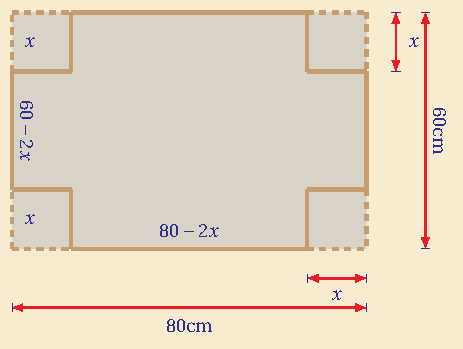
\includegraphics[scale=0.6]
{ejr-4-5-16.pdf}%
\caption{Ejemplo \ref{lacaja}}%
\label{lacaja2}%
\end{figure}
Supongamos que $x$ cent\'{\i}metros es la longitud de los cuadrados a
recortar. Las dimensiones, en $cm$, de la caja a construir son entonces:
\begin{align*}
\mbox{Largo:} &  80-2x\\
\mbox{Ancho:} &  60-2x\\
\mbox{Alto:} &  x
\end{align*}
Por lo que el volumen de la caja,en $cm^{3}$, expresado en funci\'{o}n de $x$
es:
\[
V(x)=x(80-2x)(60-2x)=2x(x-40)(x-30)=2x^{3}-140x^{2}+2400x
\]
donde el dominio \textquotedblleft pr\'{a}ctico" de la funci\'{o}n es $(0,30)$
(\textquestiondown Por qu\'{e}?). Si consideramos la funci\'{o}n en el cerrado
$[0,30]$, en el cual es continua, estamos interesados en el valor m\'{a}ximo
(positivo) de $V$. Es claro que tal m\'{a}ximo se alcanza en el abierto pues
en los extremos $V(x)=0$. Derivando tenemos
\[
V^{\prime}(x)=6x^{2}-280x+2400,
\]
de modo que la derivada es nula en
\begin{align*}
\frac{10}{3}\left(  7-\sqrt{13}\right)   &  \approx11.3148\\
\frac{10}{3}\left(  7+\sqrt{13}\right)   &  \approx35.3518
\end{align*}
de los cuales nos interesa solo $11.3148$, donde hay un m\'{a}ximo relativo.
Es para este valor aproximado que se alcanza el m\'{a}ximo volumen deseado.
\end{sol}

\begin{example}
De una l\'{a}mina circular de radio $R$ se recorta un sector circular, como el
de la f\'{\i}gura, para fabricar un cono circular recto. Determinar el
\'{a}ngulo $\theta$ para el cual el cono tenga un volumen m\'{a}ximo.%
\begin{center}
\includegraphics[scale=0.6]%
{ejr-4-5-17.pdf}%
\end{center}
\end{example}

\begin{sol}
El volumen del cono viene dado por
\begin{equation}
V=\frac{1}{3}\pi r^{2}h \label{Esc}%
\end{equation}
donde $r$ y $h$ son el radio y la altura del cono como se muestra en la
f\'{\i}gura. Note ademas que
\begin{align}
h  &  =\sqrt{R^{2}-r^{2}}\label{Esc1}\\
r  &  =\dfrac{R\theta}{2\pi}. \label{Esc2}%
\end{align}
De (\ref{Esc1}) en (\ref{Esc}) se tiene que:%
\begin{equation}
V=\frac{1}{3}\pi r^{2}\sqrt{R^{2}-r^{2}} \label{Esc3}%
\end{equation}
reemplazando finalmente (\ref{Esc2}) en (\ref{Esc3}), obtenemos $V=V\left(
\theta\right)  ,$ donde
\begin{align*}
V\left(  \theta\right)   &  =\frac{1}{3}\pi\left(  \dfrac{R\theta}{2\pi
}\right)  ^{2}\sqrt{R^{2}-\left(  \dfrac{R\theta}{2\pi}\right)  ^{2}}\\
V\left(  \theta\right)   &  =\frac{1}{24\pi^{2}}R^{3}\theta^{2}\sqrt{4\pi
^{2}-\theta^{2}}%
\end{align*}
Derivando $V\left(  \theta\right)  $ se obtiene:%
\[
\frac{dV\left(  \theta\right)  }{d\theta}=\frac{1}{24}R^{3}\theta\frac
{8\pi^{2}-3\theta^{2}}{\pi^{2}\sqrt{\left(  4\pi^{2}-\theta^{2}\right)  }}%
\]
Por lo tanto, los puntos cr\'{\i}ticos vienen dados por $\theta=0$ y
$\theta=\frac{2\pi}{3}\sqrt{6}$. Como $V\left(  \theta\right)  $ es continua
en $0\leq\theta\leq2\pi$, el teorema \ref{tvex} nos asegura la existencia de
un m\'{a}ximo y un m\'{\i}nimo para la funci\'{o}n en el intervalo. Para el
c\'{a}lculo de estos valores consideraremos la tabla siguiente
\[%
\begin{tabular}
[c]{|c|c|}\hline\hline
$x$ & $V\left(  \theta\right)  $\\\hline\hline
$0$ & $0$\\\hline
$\frac{2\pi}{3}\sqrt{6}$ & $V\left(  \frac{2\pi}{3}\sqrt{6}\right)  =\frac
{2}{27}\pi R^{3}\sqrt{3}$\\\hline
$2\pi$ & $0$\\\hline
\end{tabular}
\
\]
Entonces $V\left(  \theta\right)  $ toma su mayor valor cuando $\theta
=\frac{2\pi}{3}\sqrt{6}.$
\end{sol}

\begin{example}
Hallar las dimensiones del cilindro circular recto de m\'{a}ximo volumen que
puede incribirse en un cono circular recto de radio $R$ y altura $H.$
\end{example}

%

\begin{center}
\includegraphics[scale=0.6]%
{ejr-4-5-18.pdf}%
\end{center}
\begin{sol}
En la gr\'{a}fica se muestra una secci\'{o}n plana que contiene al eje del
cono. Sean $V$ el volumen, $h$ la altura y $r$ el radio de la base del
cilindro. El volumen $V$ en funci\'{o}n a la altura $h$ y el radio $r$ viene
dado por:%
\[
V=\pi r^{2}h\text{ },
\]


como el volumen est\'{a} en funci\'{o}n de las 2 variables, es necesario
encontrar una relaci\'{o}n entre $r$ y $h.$

Notese que $r\in\left[  0,R\right]  .$ En el caso que $r=0$ o $r=R$, se tiene
un cilindro ``degenerado'', es decir un cilindro con volumen nulo. Este mismo
resultado se puede obtener para $h\in\left[  0,H\right]  $ cuando $h=0$ y
$h=H.$

De la gr\'{a}fica de la derecha es clara la semejanza entre tri\'{a}ngulos que
permite obtener la relaci\'{o}n%
\[
\frac{H-h}{r}=\frac{H}{R}%
\]
de donde $h=-H\left(  \dfrac{r-R}{R}\right)  ,$ por lo cual
\begin{equation}
V\left(  r\right)  =-\pi r^{2}H\left(  \dfrac{r-R}{R}\right)  .
\label{vcilpco}%
\end{equation}
Derivando (\ref{vcilpco}) se tiene%
\[
V^{\prime}\left(  r\right)  =-\pi rH\frac{3r-2R}{R},
\]
por lo que los puntos cr\'{\i}ticos vienen dados por $r=0$ y $r=\frac{2}{3}R.$
Como $V\left(  r\right)  $ es continua en $\left[  0,R\right]  ,$el teorema
\ref{tvex} nos asegura la existencia de un m\'{a}ximo y un m\'{\i}nimo para la
funci\'{o}n$V$ en el intervalo. Para el c\'{a}lculo de estos valores
consideraremos la tabla siguiente
\[%
\begin{tabular}
[c]{|c|c|}\hline\hline
$r$ & $V\left(  r\right)  $\\\hline\hline
$0$ & $0$\\\hline
$\frac{2}{3}R$ & $\frac{4}{27}\pi R^{2}H$\\\hline
$R$ & $0$\\\hline
\end{tabular}
\ \
\]
Entonces $V\left(  r\right)  $ toma su mayor valor cuando $r=\frac{2}{3}R.$ Es
decir, las dimensiones del cilindro de mayor volumen que se puede incribir en
un cono de radio $R$ y altura $H$ viene dado por $r=\frac{2}{3}R$ y
$h=\frac{1}{3}H.$
\end{sol}

\section{Ejercicios propuestos}

\begin{center}
\textsc{I. Monoton\'{\i}a, Concavidad, m\'{a}ximos y m\'{\i}nimos.}
\end{center}

\begin{enumerate}
\item Determine (en caso de existir) para cada una de las funciones dadas a
continuaci\'{o}n : puntos cr\'{\i}ticos, m\'{a}ximos, m\'{\i}nimos, e
intervalos de monoton\'{\i}a.

\begin{enumerate}
\item $f\left(  x\right)  =x-\dfrac{24}{x+1}-5\ln\left(  x+1\right)  ^{2}.$

\item $f\left(  x\right)  =3x^{4}-44x^{3}+144x^{2}.$

\item $f\left(  x\right)  =x^{\frac{5}{3}}-5x^{\frac{2}{3}}.$

\item $f\left(  x\right)  =\dfrac{5x+16}{x+1}+2x.$

\item $f\left(  x\right)  =x^{3}-4x^{2}-6x+3.$

\item $f\left(  x\right)  =\left(  x^{2}-9\right)  ^{3}.$

\item $f\left(  x\right)  =\dfrac{9}{4\left(  2x+1\right)  }+\frac{9}{8}%
\ln\left(  2x+1\right)  ^{2}-\ln\left(  x+1\right)  ^{2}.$

\item $f\left(  x\right)  =xe^{\frac{-x^{2}}{8}}.$

\item $f\left(  x\right)  =x^{4}-3x^{3}+x^{2}-2.$
\end{enumerate}

\item Determine para cada una de las funciones a continuaci\'{o}n los valores
extremos en el intervalo cerrado dado.

\begin{enumerate}
\item $f\left(  x\right)  =x-\frac{24}{x+1}-5\ln\left(  x+1\right)  ^{2}$, en
$\left[  0,3\right]  .$

\item $f\left(  x\right)  =3x^{4}-44x^{3}+144x^{2}$, en $\left[  -3,4\right]
.$

\item $f\left(  x\right)  =\dfrac{5x+16}{x+1}+2x$, en $\left[  -\frac{1}%
{2},2\right]  .$

\item $f\left(  x\right)  =x^{3}-4x^{2}-6x+3$, en $\left[  -4,4\right]  .$

\item $f\left(  x\right)  =\left(  x^{2}-1\right)  ^{3}$, en $\left[
-2,1\right]  .$

\item $f\left(  x\right)  =\dfrac{9}{4\left(  2x+1\right)  }+\frac{9}{8}%
\ln\left(  2x+1\right)  ^{2}-\ln\left(  x+1\right)  ^{2}$, en $\left[
0,2\right]  .$

\item $f\left(  x\right)  =x^{3}e^{-\frac{x}{4}}$, en $\left[  -3,4\right]  .$

\item $f\left(  x\right)  =x+3\cos2x,$ en $\left[  0,\pi\right]  .$

\item $f\left(  x\right)  =e^{-\frac{1}{2}x}\left(  x^{2}+5x-2\right)  $ en
$\left[  -1,2\right]  .$
\end{enumerate}

\item Determine (en caso de existir) para cada una de las funciones dadas a
continuaci\'{o}n : puntos cr\'{\i}ticos, puntos de inflexi\'{o}n, m\'{a}ximos
y m\'{\i}nimos, intervalos de concavidad e intervalos de monoton\'{\i}a.

\begin{enumerate}
\item $f\left(  x\right)  =\dfrac{x}{2}+\cos x$, $x\in\left[  -\frac{3}{2}%
\pi,\frac{3}{2}\pi\right]  .$

\item $f\left(  x\right)  =xe^{-\frac{x^{2}}{2}}.$

\item $f\left(  x\right)  =\frac{3}{4}\left(  x^{2}-1\right)  ^{\frac{2}{3}}.$

\item $f\left(  x\right)  =5x^{\frac{2}{3}}-2x.$

\item $f\left(  x\right)  =1-9x-6x^{2}-x^{3}.$

\item $f\left(  x\right)  =2\cos x+\sin^{2}x,$ $x\in\left[  -2\pi,2\pi\right]
.$

\item $f\left(  x\right)  =\left(  x^{2}-4\right)  ^{3}.$

\item $f\left(  x\right)  =x^{2}e^{\frac{-x^{2}}{4}}.$

\item $f\left(  x\right)  =x\ln x^{2}.$

\item $f\left(  x\right)  =\frac{1}{4}x^{4}-\frac{7}{2}x^{2}+6x.$

\item $f\left(  x\right)  =e^{-\frac{1}{2}x}\left(  x^{2}+5x-2\right)  .$

\item $f\left(  x\right)  =\sqrt[3]{\left(  -x+1\right)  ^{2}}\left(
2x-1\right)  .$

\item $f\left(  x\right)  =-\dfrac{1}{\sqrt{2\pi}}e^{-\frac{x^{2}}{2}}.$

\item $f\left(  x\right)  =x^{3}e^{-x^{2}}.$
\end{enumerate}

\item Realice el bosquejo de la gr\'{a}fica de cada una de las funciones del
ejercicio 3.

Para las siguientes funciones determine

\begin{description}
\item[(i)] Intervalos de monoton\'{\i}a

\item[(ii)] Intervalos de Concavidad

\item[(iii)] Puntos cr\'{\i}ticos

\item[(iv)] Puntos de Inflexi\'{o}n

\item[(v)] Valores extremos

\item[(vi)] Dominio

\item[(vii)] Interceptos con los ejes

\item[(viii)] Asintotas
\end{description}

Construya con esta informaci\'{o}n la gr\'{a}fica de la funci\'{o}n citada y
comparela con la gr\'{a}fica dada

\begin{enumerate}
\item
$f\left(  x\right)  =\dfrac{x}{2}+\cos x,\! I=\left[  -\frac{3}{2}\pi,\frac
{3}{2}\pi\right]$  
\begin{center}
\includegraphics[scale=0.4]%
{ejp-4-6-4a.pdf}%
\end{center}
\item
$f\left(  x\right)  =xe^{-\frac{x^{2}}{2}}$
\begin{center}
%
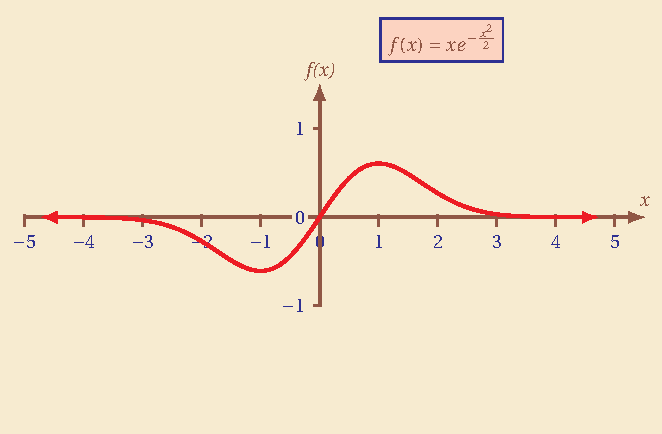
\includegraphics[scale=0.7]
{ejp-4-6-4b.pdf}%
\end{center}

\item
$f\left(  x\right)  =5x^{\frac{2}{3}}-2x$
\begin{center}
%
\includegraphics[scale=0.6]%
{ejp-4-6-4c.pdf}%
\end{center}

\item
$f\left(  x\right)  =1-9x-6x^{2}-x^{3}$
\begin{center}
%
\includegraphics[scale=0.6]%
{ejp-4-6-4d.pdf}%
\end{center}

\item
$f\left(  x\right)  =\left(  x\left(  8-x\right)  \right)  ^{\frac{2}{3}}$
\begin{center}
%
\includegraphics[scale=0.6]%
{ejp-4-6-4e.pdf}%
\end{center}

\item
$f\left(  x\right)  =2\cos x+\sin^{2}x,I=\left[  -2\pi,2\pi\right]  $
\begin{center}
%
\includegraphics[scale=0.6]%
{ejp-4-6-4f.pdf}%
\end{center}

\item
$f\left(  x\right)  =\left(  x^{2}-4\right)  ^{3}$
\begin{center}
%
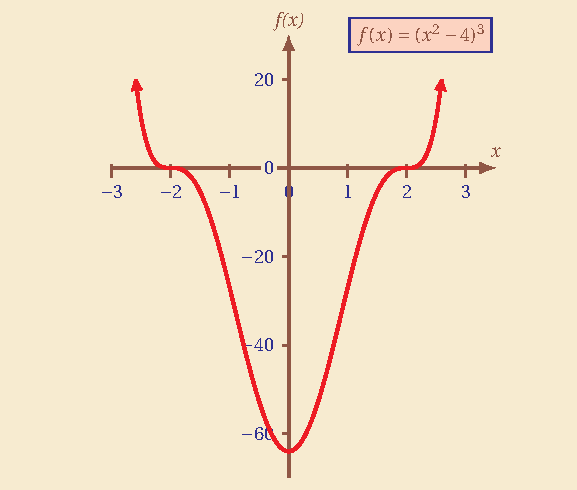
\includegraphics[scale=0.6]
{ejp-4-6-4g.pdf}%
\end{center}


\item
$f\left(  x\right)  =x^{2}e^{\frac{-x^{2}}{4}}$
\begin{center}
%
\includegraphics[scale=0.6]%
{ejp-4-6-4h.pdf}%
\end{center}

\item
$f\left(  x\right)  =x\ln x^{2}$
\begin{center}
%
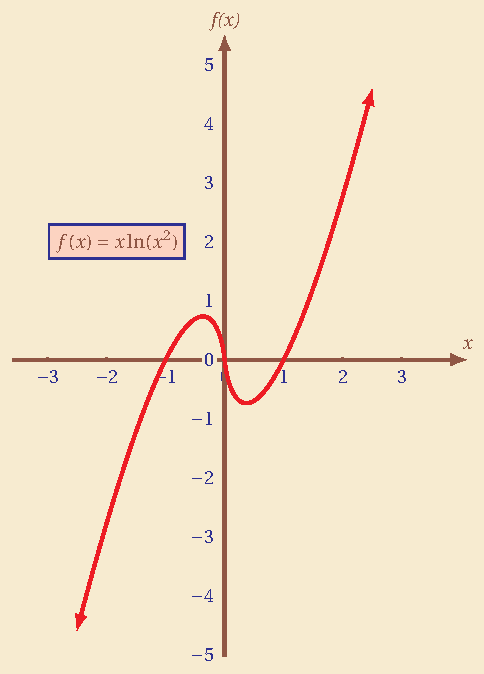
\includegraphics[scale=0.5]
{ejp-4-6-4i.pdf}%
\end{center}

\item  %TODO  
$f\left(  x\right)  =\frac{1}{4}x^{4}-\frac{7}{2}x^{2}+6x$
\begin{center}
%
\includegraphics[scale=0.5]%
{ejp-4-6-4j.pdf}
\end{center}%

\end{enumerate}

\item Sea
\[
g\left(  x\right)  =x^{3}+bx^{2}+cx+d
\]
Obtenga valores para $b,c$ y $d$ tal que se cumplan las siguientes tres condiciones:

\begin{itemize}
\item[i.] La grafica de la funci\'{o}n $g\left(  x\right)  $ contenga al punto
$A(2,2)$

\item[ii] $g\left(  x\right)  $ tenga un valor extremo en $x=4$

\item[ii.] $g\left(  x\right)  $ tenga un punto de inflexi\'{o}n en $x=2.$
\end{itemize}
\end{enumerate}

\begin{center}
\textsc{II. Razones relacionadas}
\end{center}

\begin{enumerate}
\item Si $2\operatorname{sen}x+4\tan y=3$ y $\dfrac{dy}{dt}=3,$ halle
$\dfrac{dx}{dt}$ en $\left(  \frac{1}{6}\pi,\frac{1}{3}\pi\right)  .$

\item Si $y\left(  \operatorname{sen}x+1\right)  =4$ y $\dfrac{dy}{dt}=-4,$
obtenga $\dfrac{dx}{dt}$ en $x=-\pi$

\item Si $s^{2}=x^{2}+y^{2}+3xy,s^{3}=7y^{2}-2x^{2}$ y $\dfrac{dy}{dt}=-2$.
Obtenga $\dfrac{ds}{dt}$ y $\dfrac{dx}{dt}$ cuando $\left(  x,y\right)
=\left(  1,1\right)  .$

\item Si $s^{2}=x\sin\theta,x^{2}+\cos^{2}\theta=2\theta,$ y $\dfrac
{dx}{d\theta}=\dfrac{1}{4}.$ Entonces calcule $\dfrac{ds}{d\theta}$ cuando
$\theta=\frac{\pi}{2}.$

\item Un punto $P$ se mueve, en sentido antihorario, sobre la circunferencia
$x^{2}+y^{2}=25.$ La distancia del punto a $\left(  -7,-7\right)  $ varia a
raz\'{o}n de $\frac{1}{2}$ unidad por segundo. Determine la raz\'{o}n a la
cual varian las coordenadas $x$ e $y$ cuando $\left(  x,y\right)  =\left(
-3,4\right)  .$

\item Un punto $P$ se mueve, en sentido horario, sobre la par\'{a}bola
$\left(  x-2\right)  ^{2}=-16\left(  y+5\right)  .$ La distancia del punto a
$\left(  0,-1\right)  $ varia a raz\'{o}n de $\frac{1}{3}$ unidad por segundo.
Determine la raz\'{o}n a la cual varian las coordenadas $x$ e $y$ cuando
$\left(  x,y\right)  =\left(  1,-\frac{81}{16}\right)  .$

\item \label{cap4prob7}Una v\'{\i}a de ferrocarril cruza una carretera
formandose un \'{a}ngulo de $60^{0}$, como lo muestra la figura$.$ Una
locomotora a $500$ metros de la intersecci\'{o}n se aleja de ella a raz\'{o}n
de $100\dfrac{km}{h}.$ Un automovil a $200$ metros de la intersecci\'{o}n se
acerca a ella a raz\'{o}n de $80\dfrac{km}{h}$ \textquestiondown Cu\'{a}l es
la variaci\'{o}n de la distancia entre la locomotora y el automovil?%

\begin{figure}[H]
\begin{center}
\includegraphics[scale=0.6]%
{ejp-4-6-7.pdf}%
\caption{Problema \ref{cap4prob7}.}%
\label{problematren}%
\end{center}
\end{figure}



\item \label{cap4prob8}Cierta cantidad de aceite fluye hacia el interior de un
deposito en forma de cono invertido a raz\'{o}n de $0.1\pi\,\frac{m^{3}}{\min
}.$ El deposito tiene un radio de 2.5 m en su parte superior y una profundidad
de 10 m. Si el deposito inicialmente tenia una peque\~{n}a cantidad de aceite,
\textquestiondown Qu\'{e} tan rapido cambia la altura del l\'{\i}quido, cuando
est\'{e} alcanza una altura de $8m$ en en interior del deposito?.%

\begin{figure}[H]
\centering
\includegraphics[scale=0.4]%
{ejp-4-6-8op.pdf}%
\caption{Problema \ref{cap4prob8}.}%
\label{figuraej8}%
\end{figure}


\item Una piedra es arrojada a un estanque tranquilo. Una serie de anillos
circulares conc\'{e}ntricos se extienden por el estanque y el radio de la
regi\'{o}n perturbada aumenta a raz\'{o}n de $4\dfrac{cm}{s}$.
\textquestiondown Con qu\'{e} rapidez aumenta dicha \'{a}rea cuando el radio
es de 4 cm?

\item Una escalera de 6 metros de longitud est\'{a} recargada sobre una rampa
que esta inclinada $60^{0}$ respecto de la horizontal. Si la base de la
escalera se esta resbalando a raz\'{o}n de $\frac{1}{20}\dfrac{m}{s},$
\textquestiondown Con qu\'{e} rapidez se desplazar\'{a} la parte superior de
la escalera cuando su base est\'{e} a 3 metros de la rampa?

\item Una antena de radar est\'{a} instalada en un barco situado a 7
kilometros de una costa recta, y gira a 32 rpm. \textquestiondown Con qu\'{e}
rapidez se desplaza el haz del radar a lo largo de la l\'{\i}nea costera
cuando dicho haz forma un \'{a}ngulo de $45^{0}$ con la citada l\'{\i}nea?

\item \label{cap4prob12}Un hombre de 1.80 m de estatura camina hacia un
edificio a una velocidad de $\frac{2}{3}\dfrac{m}{s}$. Si hay una luz en el
piso, que ilumina la fachada, localizada a 10 metros del edificio
\textquestiondown Con qu\'{e} rapidez se acorta la sombra de la persona
proyectada sobre la fachada cuando se encuentra a 4 metros de la
edificaci\'{o}n?.%

\begin{figure}[H]
\centering
\includegraphics[scale=2.5]%
{ejp-4-6-12.pdf}%
\caption{Problema \ref{cap4prob12}.}%
\label{ejemplo12}%
\end{figure}



\item Una escalera de $3m$ de largo resbala sobre una pared vertical. Si su
base se aleja de la pared a raz\'{o}n constante de $2m$ por segundo,
\textquestiondown a qu\'{e} velocidad resbala el extremo superior de la
escalera sobre la pared cuando la distancia de la base de la escalera a la
pared es de $1m$ ?

\item Una part\'{\i}cula m\'{o}vil se desplaza en el plano siguiendo una
trayectoria circular de ecuaci\'{o}n $x^{2}+y^{2}=1$. Si la abscisa cambia a
una raz\'{o}n de $2x$ unidades por segundo \textquestiondown c\'{o}mo
var\'{\i}a su ordenada cuando la part\'{\i}cula est\'{a} en el punto
$(\frac{1}{2},\frac{\sqrt{3}}{2})$?

\item El \'{a}rea de un cuadrado decrece a raz\'{o}n de $1.5cm^{2}$ por
segundo. Encuentre la raz\'{o}n de cambio de la longitud de los lados cuando
el \'{a}rea es de $100cm^{2}$. \textquestiondown C\'{o}mo est\'{a} cambiando,
en ese momento el \'{a}rea con relaci\'{o}n a la longitud de los lados?

\item Un bal\'{o}n esf\'{e}rico pierde volumen, sin perder su forma
esf\'{e}rica, a raz\'{o}n constante de $10\ cm^{3}$ por minuto.
\textquestiondown C\'{o}mo disminuye su radio? \textquestiondown Cu\'{a}l es
la raz\'{o}n de cambio del mismo cuando el volumen es de $60cm^{3}$?.

\item Un perro se encuentra entrenando sobre una pista par\'{a}bolica de
ecuaci\'{o}n
\[
y=3x^{2}-2x-2.
\]
Su amo se encuentra, en una caseta de observaci\'{o}n, en la posici\'{o}n
$\left(  2,10\right)  $ y quiere determinar si su perro puede seguir en las
carreras o se convierte en la mascota de sus hijos. La prueba consiste en
medir la rapidez vertical del perro en el punto final de la pista. La rapidez
vertical m\'{\i}nima exigida es de $1.3\frac{m}{s}.$ Si el recorrido se inicia
en la posici\'{o}n $\left(  -3,31\right)  $ y termina en la posici\'{o}n
$\left(  2,6\right)  $, y durante todo el recorrido la distancia a su
due\~{n}o tiene una variaci\'{o}n constante de $1.4\frac{m}{s}.$
\textquestiondown El perro pasa la prueba?.

\begin{center}
\includegraphics[scale=0.6]%
{ejp-4-6-17.pdf}%
\end{center}



\item Un deposito de agua con forma de prisma recto con secciones
transversales tri\'{a}ngulos is\'{o}sceles ,como el de la figura, es
alimentado por una manguera de la cual fluye agua a raz\'{o}n de
$1.8\frac{m^{3}}{\min}$. El deposito tambien presenta un escape del cual fluye
agua a raz\'{o}n de $0.22\frac{m^{3}}{\min}.$ \textquestiondown Qu\'{e} tan
rapido aumenta el nivel del agua (en $\frac{m}{\min}$),en el instante en que
la altura del agua es $2$ $m$?%
\begin{center}
\includegraphics[scale=0.4]%
{ejp-4-5-18op.pdf}%
\end{center}

\end{enumerate}

\begin{center}
\textsc{III. Optimizaci\'{o}n.}
\end{center}

\begin{enumerate}
\item Sea $\triangle ABC$ is\'{o}sceles con $AB=AC.$ Si $m\measuredangle
BAC=\alpha,$ obtenga el valor del \'{a}ngulo $\alpha$ tal que el \'{a}rea del
$\triangle ABC$ sea m\'{a}xima.

\item Determine dos n\'{u}meros positivos cuya suma sea $100$ y cuyo producto
sea m\'{a}ximo.

\item Una isla est\'{a} ubicada en el punto $A$, $4\,km$ mar adentro del punto
m\'{a}s cercano $B$ de una playa recta. Una atleta, en la isla desea ir al
punto $C$, a $6$ $km$ de $B$ playa abajo. La mujer puede dirigirse hacia el
punto $P$, entre $B$ y $C$, en un bote de remos a $3.5\dfrac{km}{h}$ y
desp\'{u}es caminar en forma recta de $P$ a $C$ a $6\dfrac{km}{h}.$
\textquestiondown Donde debe estar el punto $P$ (respecto a $B$) para que la
mujer se desplace en el menor tiempo posible?
\begin{center}
\includegraphics[scale=1]%
{ejp-4-6-3op.pdf}%
\end{center}

\item Determine el \'{a}rea del rect\'{a}ngulo m\'{a}s grande que tenga dos
v\'{e}rtices en el eje $x$ y los otros dos en la par\'{a}bola $y=16-x^{2},$
por arriba del eje $x.$

\item Determine la distancia m\'{\i}nima desde el punto $P\left(  1,0\right)
$ a un punto de la curva $y^{2}-x^{2}=9,$ y encuentre el punto de la curva
m\'{a}s cercano a $P.$

\item Pruebe que la distancia m\'{\i}nima desde el punto $P_{1}\left(
x_{1},y_{1}\right)  $ a la recta $l$ que tiene la ecuaci\'{o}n
\[
Ax+By+C=0
\]
esta dada por
\[
\dfrac{\left\vert Ax_{1}+By_{1}+C\right\vert }{\sqrt{A^{2}+B^{2}}}%
\]


\item Determine las dimensiones del cilindro con mayor volumen que pueda
inscribirse en un cono circular recto que tiene radio $R$ y altura $H.$

\item Un trozo de alambre de 80 centimetros de longitud se dobla en forma de
rect\'{a}ngulo. Determine las dimensiones del rect\'{a}ngulo de mayor \'{a}rea posible.

\item Una p\'{a}gina debe contener 150 centimetros cuadrados de material
impreso con 4 centimetros de margen superior e inferior y 2 centimetros de
margen derecho e izquierdo \textquestiondown Qu\'{e} dimensiones debe tener la
p\'{a}gina para que gaste menos papel?

\item Si se corta un alambre de 10 metros de longitud y se quiere formar un
rectangulo y una circunferencia \textquestiondown Donde debe cortarse el
alambre para que el \'{a}rea de las figuras combinadas sea m\'{a}xima.

\item Hay que construir una pileta de las dimensiones que se muestran.
S\'{o}lo se puede variar el \'{a}ngulo $\theta$ . \textquestiondown Con
qu\'{e} \'{a}ngulo se obtendr\'{a} el volumen m\'{a}ximo de la pileta?%
\begin{center}
\includegraphics[scale=0.4]%
{ejp-4-5-11op.pdf}%
\end{center}



\item Dos lados de un tri\'{a}ngulo tienen $a$ y $b$ de largo, y el \'{a}ngulo
entre ellos es $\theta.$ \textquestiondown Que valor de $\theta$
maximizar\'{a} el \'{a}rea del tri\'{a}ngulo?

\item Un granjero desea cercar tres terrenos rectangulares adyacentes
identicos, cada uno de ellos de 1800 pies cuadrados de \'{a}rea, incluyendo
cerca en medio de ellos. \textquestiondown Cu\'{a}les ser\'{\i}an las
dimensiones de los terrenos para emplear la menor cantidad de cerca posible?

\item Dada una esfera de radio $R$. Calcular en funci\'{o}n de $R$, el radio
$r$ y la altura $h$ del cono circular recto de mayor volumen que puede
inscribirse en la esfera.

\item Obtenga una ecuaci\'{o}n de la recta tangente a la curva
\[
y=\frac{1}{3}x^{3}+2x^{2}+5x-2
\]
cuya pendiente sea m\'{\i}nima

\item Si $a$ y $b$ son los catetos de un tri\'{a}ngulo rect\'{a}ngulo cuya
hipotenusa es $4$, hallar el mayor valor de $a^{2}+3b^{2}-5a+2.$

\item Dos f\'{a}bricas est\'{a}n situadas en las coordenadas $\left(
-3,0\right)  $ y $\left(  3,0\right)  $ y su central de suministro de
energ\'{\i}a en el punto $\left(  0,8\right)  .$ Determine donde debe
colocarse el punto $A$, tal que la longitud de conducci\'{o}n de la
energ\'{\i}a a las dos f\'{a}bricas sea m\'{\i}nima.%
\begin{center}
\includegraphics[scale=0.6]%
{ejp-4-6-17op.pdf}%
\end{center}


\item Una ventana tiene forma de rect\'{a}ngulo terminado por un semicirculo
de di\'{a}metro igual a la base del rect\'{a}ngulo. La parte circular ha de
ser de cristal transparente y la parte rectangular ha de ser de cristales de
color que admite solo dos tercios de la luz por metro cuadrado que el cristal
transparente. El perimetro total de la ventana ha de tener longitud fija $25$
m. Hallar las dimensiones de la ventana que deja pasar la mayor cantidad
posible de luz.

\item Hallar la menor distancia de $\left(  0,6\right)  $ del eje $Y$ a la
par\'{a}bola $x^{2}=4y.$

\item Considere la circunferencia de ecuaci\'{o}n
\[
x^{2}+y^{2}-2x+2y+1=0.
\]
Encuentre los puntos de la misma que est\'{a}n m\'{a}s cerca y m\'{a}s lejos
del origen del sistema de coordenadas.

\item Una caja cerrada de base cuadrada debe tener un volumen de $1000$
$cm^{3}.$ El material del fondo de la tapa de la caja tiene un costo de 0.3
euros por $cm^{2}$ y el material de los laterales cuesta $0.15$ euros por
$cm^{2}.$ Determine las dimensiones de la caja para que el costo total sea m\'{\i}nimo.

\item Se dobla la esquina superior izquierda de un trozo de papel de 8
pulgadas de ancho por 12 pulgadas de largo para llevarla hasta el borde de la
derecha, como en la figura. \textquestiondown Com\'{o} se doblar\'{\i}a de
modo que se minimice la longitud de doblez?. En otras palabras
\textquestiondown Como elegir\'{\i}a $x$ para minimizar $y$?%

\begin{center}
\includegraphics[scale=0.4]%
{pagina-doblada.pdf}%
\end{center}


\end{enumerate}

